\onecolumn

\tableofcontents

\section{Applications of orthogonal convolutions}\label{sec:ap_intro}

    Orthogonal layers have become fundamental components in various deep learning architectures due to their unique mathematical properties, which benefit multiple applications.
    
    \paragraph{Provable Robustness with 1-Lipschitz Networks.}
    Ensuring robustness against adversarial attacks is a critical challenge. Early work in this field \cite{szegedy_intriguing_2013} identified a link between a network's adversarial robustness and its Lipschitz constant, which led to the development of networks with a Lipschitz constant of one (1-Lipschitz networks). Initially, regularization techniques were used \cite{cisse2017parseval}, but interest in constrained networks quickly grew. Orthogonal layers, in particular, have an inherent Lipschitz constant of one, as they preserve the input norm through each transformation. This property is instrumental in achieving provable robustness by allowing for certified bounds on the network's output perturbations in response to adversarial inputs \cite{anil_sorting_2019}. By controlling the network's sensitivity to input changes, orthogonal layers play a crucial role in building models resilient to adversarial manipulations.
    Besides robustness, Lipschitz-constrained networks have diverse applications: they are closely linked to WGANs and optimal transport \cite{arjovsky2017wasserstein, bethune2024deep}, enable scalable differential privacy \cite{bethunedp}, allow conformal prediction in adversarial setting \cite{massena2025efficient}, and prevent singularities in diffusion models \cite{yang2023lipschitz}. Additionally, they guarantee the existence and uniqueness of solutions in classification \cite{bethune_pay_2022} and flow-matching networks \cite{perko2013differential, coddington1956theory}.
    
    \paragraph{Enhancing Performance in Normalizing Flows.}
    Normalizing flows are a class of generative models that transform simple probability distributions into complex ones through a series of invertible and differentiable mappings. Although they have different objectives, this domain intersects with the field of provable adversarial robustness. For instance, \cite{dinh2016density, rezende2015variational} employs a channel masking scheme, which was later used to emulate striding in Lipschitz layers designed for adversarial robustness. Separately, Lipschitz layers can be applied to build invertible residual networks \cite{behrmann2019invertible}. In both fields, orthogonal convolutions are essential, as they facilitate the construction of invertible transformations with tractable Jacobian determinants. The use of orthogonal layers ensures that the Jacobian determinant is constant or easily computable, simplifying likelihood estimation during training \cite{kingma2018glow}. This property enables efficient and stable training of normalizing flow models, leading to improved performance in density estimation and generative tasks.
    
    \paragraph{Stabilizing Training in Deep and Recurrent Neural Networks.}
    Training recurrent neural networks (RNNs) involves propagating gradients through time, which can lead to vanishing or exploding gradients due to the multiplicative nature of sequential weight applications. Orthogonal weight matrices in RNNs help preserve the gradient norm across time steps, thus preventing degradation of the learning signal \cite{kiani_projunn_2022}. By constraining recurrent weights to be orthogonal, the network maintains a consistent flow of information, enabling it to capture long-term dependencies more effectively. This stabilization is essential for tasks requiring understanding long-range dependencies in time series, such as language modeling and speech recognition. These approaches also facilitate the training of very deep networks \cite{qi_deep_isometric_2020} with improved generalization properties \cite{bansal2018gainorthogonalityregularizationstraining}.
    
    \paragraph{Improving Stability in Wasserstein Generative Adversarial Networks.}
    Generative Adversarial Networks (GANs) are powerful models for generating realistic data, but they often suffer from training instability. Wasserstein GANs (WGANs) \cite{arjovsky2017wasserstein} address this issue by optimizing the Wasserstein distance between the real and generated data distributions. A key requirement for WGANs is that the discriminator (or critic) function must be Lipschitz continuous. Orthogonal layers naturally satisfy this Lipschitz condition, eliminating the need for techniques like weight clipping or gradient penalties \cite{gulrajani2017improved}, which can adversely affect training dynamics. By incorporating orthogonal convolutions into the discriminator, WGANs achieve more stable training \cite{miyato2018spectral, muller2019orthogonal} and produce higher-quality generative results. Orthogonality has been integral to the successful scaling of GAN training \cite{brock2018large}. %\textbf{https://github.com/ezqlwyb/GAN}

\paragraph{Extending the applicability of Proximal Neural Networks.}
Proximal Neural Networks (PNNs) offer a principled approach to designing and training deep architectures by drawing inspiration from optimization theory—specifically, proximal algorithms and $\alpha$-averaged operators \cite{hasannasab2020parseval, combettes2020lipschitz}. A central insight in this framework is the emergence and enforcement of orthogonality in learned operators, which can improve network stability. \cite{hertrich2021convolutional} proposes an extension to convolutional operators but notes that, for limited kernel sizes, optimizing on the manifold is challenging and instead relies on penalization, similar to \cite{wang_orthogonal_2020}. Using our method, AOC, and its transpose could overcome this limitation.

\section{BCOP and SC-Fac re-explained with our framework}\label{ap:BCOP_detail}
In this section, we  outline the key steps in constructing orthogonal convolutions using  the BCOP (\cref{fig:method_bigpic}) or SC-Fac methods within the framework established in the paper.

    \paragraph{From Orthogonal Matrices to Orthogonal $c_o \times c_i\times 1 \times 1$ Convolutions.}  
    \todo{The core methods are cited without explanation, making this paper not self-contained. This may be resolved if the authors wish to briefly describe methods such as Björk-Bowie iterative refinement, exponential parametrization, Cayley, QR factorization, RKO, etc...}
    A substantial body of research exists on building orthogonal matrices $M \in \RR^{c_o \times c_i}$. One common approach involves applying a differentiable projection operator to an unconstrained weight matrix, yielding an orthogonal matrix such that $M M^T = I$ or $M^T M = I$. Various methods exist, including the Björck and Bowie orthogonalization scheme \cite{bjorck1971iterative}, the exponential method \cite{singla_skew_2021}, the Cayley method \cite{trockman_orthogonalizing_2021}, and QR factorization \cite{van2018sylvester}. An orthogonal matrix can easily be reshaped into a convolution kernel with a $1 \times 1$ kernel $\kernel{M} \in \RR^{c_o \times c_i \times 1 \times 1}$, and such a convolution is orthogonal if $M$ is orthogonal. These convolutions are mainly used to change the number of channels (\cref{fig:method_bigpic}-1).
    
    %\paragraph{From Matrices to $1 \times 2$ Orthogonal Convolutions.}
    \paragraph{Building $c\times c \times 1 \times 2$ Orthogonal Convolutions.}
    Stacking two orthogonal $1\times 1$ convolution kernels along their last dimensions\footnote{Done in practice with \texttt{torch.stack([K\_1, K\_2], axis=-1)}} leads to a $1 \times 2$ convolution, though it is generally not orthogonal. Authors of \cite{xiao_dynamical_2018, su_scaling-up_2021} noted that additional constraints are needed, proposing a half-rank symmetric projector to construct a $1 \times 2$ orthogonal convolution: from a column-orthogonal matrix $M \in \RR^{c \times \frac{c}{2}}$\footnote{This implies that $c\geq2$. When $c$ is even, $\lfloor\frac{c}{2}\rfloor$ is used in practice}, the matrix $N = M M^T \in \RR^{c \times c}$ is a symmetric projector that satisfies:
        \[
            N = N^2 = N^T \quad \text{and} \quad (I - N) = (I - N)^2 = (I - N)^T
        \]
    These two matrices can be reshaped into $c \times c \times 1 \times 1$ convolution kernels, and stacking them along the last dimension results in an orthogonal $c \times c \times 1 \times 2$ convolution kernel:
        \[
        \kernel{P} = \mathtt{stack(}[\kernel{N}, \kernel{I - N}]\mathtt{, axis=-1)} \Rightarrow \kernel{P} \mathbconv \kernel{P}^T = \kernel{I}
        \]
    Similarly, stacking along the penultimate dimension, $\kernel{Q} = \mathtt{stack([N, I - N], axis=-2)}$, results in an orthogonal $c \times c \times 2 \times 1$ kernel. 
    % \franck{est ce qu'il faut que c soit divisible par 2?} 
    Although already proven by previous work, proof of this can be found in \cref{sec:ap_1x2_ortho}.
    
    \paragraph{From $1 \times 2$ to $k_1 \times k_2$ Orthogonal Convolutions.}  
    The three papers propose to build standard orthogonal convolutions by composing smaller kernels based on the following properties:
    

    
    Using \Bconv, we can represent the composition of $1 \times 2$ and $2 \times 1$ kernels\footnote{As indicated in \cref{def:orthogonal}, $k_1$ and $k_2$ parameters do not affect row or column orthogonality} to obtain a kernel with any desired shape. The differences among the three approaches lie in the composition order:  
    Authors of \cite{su_scaling-up_2021} chose to compose $(k_1-1)$ $2 \times 1$ kernels $\kernel{P_i}$, followed by a $1 \times 1$ kernel $\kernel{M}$, and $(k_2-1)$ $1 \times 2$ kernels $\kernel{Q_i}$ to form a $k_1 \times k_2$ kernel:
    \[
        \kernel{K}_{\text{\tiny{SC-Fac}}} = \underbrace{\kernel{P_{k_1-1}} \mathbconv \dots \mathbconv \kernel{P_1}}_{\text{all 1x2 kernels}} \mathbconv \underbrace{\kernel{M}}_{\text{1x1}} \mathbconv \underbrace{\kernel{Q_1} \mathbconv \dots \mathbconv \kernel{Q_{k_2-1}}}_{\text{all 2x1 kernels}}
    \]
    On the other hand, authors of \cite{li_preventing_2019}\cite{xiao_dynamical_2018} alternated $2 \times 1$ and $1 \times 2$ kernels, ending with a $1 \times 1$ convolution:
    \[
        \kernel{K}_{\text{\tiny{BCOP}}} = \underbrace{(\kernel{P_{k-1}} \mathbconv \kernel{Q_{k-1}})}_{\text{pairs of 1x2 and 2x1 kernels}} \mathbconv \dots \mathbconv (\kernel{P_1} \mathbconv \kernel{Q_1}) \mathbconv \underbrace{\kernel{M}}_{\text{1x1}}
    \]
    Both approaches have incomplete parametrizations: the first is limited to separable convolutions, while the second shows counterexamples in the general 2D convolution case. However, both methods use the same number of parameters for a given kernel size. Building a complete parametrization of 2D convolutions remains an open question, discussed in \cref{sec:ap_incomplete}. We thus base our work on the BCOP parametrization \cite{li_preventing_2019} for two main reasons: (1) any $2 \times 2$ convolution not parametrizable by BCOP can be represented with a $3 \times 3$ kernel -- a feasible solution given the trend toward larger kernels \cite{trockman_patches_2022,ding_scaling_2022}; (2) BCOP enables a faster and less memory-intensive implementation (see \cref{sec:implem}), unlocking larger networks that compensate for any potential expressiveness loss.%; and (3) the authors investigated optimization dynamics, ensuring practical layer optimization.

\section{Impact of the orthogonalization scheme on AOC}\label{ap:tech_details}

    In this section we will discuss on of the design choices for AOC: the orthogonalization procedure. Many approaches exists and we will describe the main approaches:

    \subsection{Non exhaustive list of orthogonalization methods}

    \subsubsection{QR Factorization via Modified Gram-Schmidt}

        The QR factorization is obtained using the Modified Gram-Schmidt (MGS) algorithm, as initially proposed in \cite{LaPlace1820}. The MGS procedure follows the same fundamental computational steps as the classical Gram-Schmidt method; however, it executes these steps in a different order. In classical Gram-Schmidt, each iteration involves computing a sum that includes all previously computed vectors. Conversely, the modified version corrects numerical errors at each step, leading to improved numerical stability.
        
        \begin{algorithm}   
        \begin{algorithmic}[1]
        \Require $W = [w_i]_{i\in[0,C-1]}  \in \mathbb{R}^{C\times C}$ 
        \Ensure $W= QR$, where $Q\in\mathbb{O}(C)$ is an orthogonal matrix and $R\in \mathbb{R}^{C\times C}$ is an upper triangular matrix.
        \Procedure{Modified Gram-Schmidt}{$W$}
        \State $w^c_i = w_i$, $\forall i\in[0,C-1]$ \Comment{Initialize with a copy of $W$}
        \For {$j\in range(C)$} 
            \State $r_{j,j} = \|w^c_j\|_2$
            \State $q_j = w^c_j/r_{j,j}$
            \For {$k\in range(j+1,C)$} 
                \State $r_{j,k} = q_j^T w^c_k$
                \State $w^c_k = w^c_k - r_{j,k} q_j$
            \EndFor
        \EndFor
        \State \textbf{return} $QR$
        \EndProcedure
        \end{algorithmic}
        \caption{QR Factorization via Modified Gram-Schmidt}   \label{alg:MGS} 
        \end{algorithm}
        
        %While PyTorch provides an implementation of QR factorization, empirical results indicate that its performance during neural network training is suboptimal. To improve the numerical stability of the decomposition, we apply an additional stabilization technique: an element-wise multiplication of the matrix $Q$ by the sign of the diagonal elements of $R$. This transformation ensures that the diagonal elements of $R$ remain positive, thereby enforcing the uniqueness of the decomposition and contributing to numerical stability.
        
    \subsubsection{Cayley Transform}
        
        The Cayley transform \cite{Cayley_1846} provides an alternative approach for constructing orthogonal matrices. It exploits the bijective relationship between the special orthogonal matrices $Q$ (i.e., orthogonal matrices with determinant $+1$) and skew-symmetric matrices $A$ (satisfying $A^T = -A$). The transformation is defined as follows:
        \begin{equation}\label{eq:cayley}
        Q = (I - A)(I + A)^{-1} \quad \text{or} \quad Q = (I + A)^{-1}(I - A).
        \end{equation}
        
        A matrix $A$ can be naively constructed as a skew-symmetric matrix using:
        \begin{equation}
            A = M^T - M.
        \end{equation}
        
        The extension of the Cayley transform to rectangular matrices is detailed in \cite{pauli2023lipschitz} and is formalized in  \cref{alg:cayley}.
        
        \begin{algorithm} 
        \begin{algorithmic}[1] 
        \Require $W\in \mathbb{R}^{M\times C}$, where $M>C$
        \Ensure $\hat{W}\in \mathbb{R}^{M\times C}$, an orthogonal matrix
        \Procedure{Cayley Transform}{$W$}
        \State $U,V = W[:C,:],W[C:,:]$ \Comment{Partition $W$ such that $U\in \mathbb{R}^{C\times C}$ and $V\in \mathbb{R}^{(M-C)\times C}$}
        \State $A = U - U^T + V^T V$ \Comment{Note: $A$ is not strictly skew-symmetric}
        \State $B = (I + A)^{-1}$
        \State $\hat{W_1} = B (I - A)$  \Comment{$\hat{W_1}\in \mathbb{R}^{C\times C}$}
        \State $\hat{W_2} = -2 V B$ \Comment{$\hat{W_2}\in \mathbb{R}^{(M-C)\times C}$}
        \State $\hat{W} =  [\hat{W_1}, \hat{W_2}]$  \Comment{Concatenation yields $\hat{W} \in \mathbb{R}^{M\times C}$}
        \State \textbf{return} $\hat{W}$
        \EndProcedure
        \end{algorithmic}
        \caption{Cayley Transform Algorithm}   \label{alg:cayley}   
        \end{algorithm}
        
        This approach involves matrix inversion, which can be computationally expensive, particularly for large matrices.
        
    \subsubsection{Exponential Map}
        
        The exponential map \cite{singla_skew_2021} is another technique used to generate orthogonal matrices, leveraging the properties of skew-symmetric matrices. The matrix exponential of $A$ is defined as:
        \begin{equation}
            \exp(A) = \sum_{k=0}^{\infty} \frac{A^k}{k!}.
        \end{equation}
        
        For a skew-symmetric matrix $A$, it can be shown that:
        \begin{equation}
            (e^A)^T = e^{-A}.
        \end{equation}
        Since the product of a matrix and its transpose is the identity matrix, this ensures that $e^A$ is orthogonal.
        
        In practice, numerical computations only approximate the exponential function by summing a finite number of terms. %PyTorch’s default implementation does not allow specifying the number of terms, leading to inaccuracies in achieving orthogonality. To mitigate this issue, we introduce  
        \Cref{alg:EXP} describes the Exponential Map with a spectral normalization to prevent floating-point overflows.
        
        \begin{algorithm}   
        \begin{algorithmic}[1]
        \Require $W\in \mathbb{R}^{C\times C}$, $p \in \mathbb{N}$ (number of terms in the expansion)
        \Ensure $\hat{W}\in \mathbb{R}^{C\times C}$, an orthogonal matrix
        \Procedure{Lipschitz Exponential}{$W$}
        \State $A = W - W^{T}$
        \State $\hat{A} = A / \|A\|_2$ \Comment{Spectral normalization}
        \State $\hat{W} = I_{C}, \hat{A}_{k} = I_{C}$
        \For {$j\in range(1,p)$} 
            \State $\hat{A}_{k} = \frac{\hat{A}_{k}}{k} \times \hat{A}$
            \State $\hat{W} = \hat{W} + \hat{A}_{k}$
        \EndFor
        \State \textbf{return} $\hat{W}$
        \EndProcedure
        \end{algorithmic}
        \caption{Exponential Map Algorithm}   \label{alg:EXP}   
        \end{algorithm}
        
        This method parametrizes only the special orthogonal group. The proof follows from the determinant properties of matrix exponentiation.
        
    \subsubsection{Cholesky Decomposition}
        
        The Cholesky decomposition %\cite{Cho_math} 
        has also been employed for orthogonalization \cite{hu_recipe_2023}. Given a weight matrix $M$, we construct the covariance matrix:
        \begin{equation}
            C = M M^T.
        \end{equation}
        Since $C$ is positive semi-definite by construction, its Cholesky decomposition exists:
        \begin{equation}
            C = L L^T.
        \end{equation}
        Solving the triangular system $L W = M$ yields an orthogonal matrix $W$. To ensure the positive-definiteness of $C$, a small positive perturbation is added before decomposition \cite{hu_recipe_2023}.
        
        This method is computationally efficient, provided that numerical stability is carefully managed.

    \subsubsection{Björck and Bowie}
        \cite{bjorck1971iterative} proposed an iterative algorithm for computing the best orthogonal approximation of a given matrix. This process relies solely on matrix multiplications:
        
        \[
            W_{t+1} = (1+\beta) W_t + \beta W_tW_t^\top W_t.
        \]
        
        This algorithm corresponds to the gradient descent of the regularization term \( \| WW^\top - I\|_2 \) with a learning rate of \( \beta \). The convergence radius is 1, determined by the spectral norm of \( W \). To ensure numerical stability, our implementation applies spectral normalization to the matrix. Under these conditions, \( \beta \) can be increased to its theoretical maximum of \( \frac{1}{2} \), which accelerates convergence.
        
        This specific setting allows for rapid convergence of the algorithm, requiring only 25 iterations, as demonstrated in \cite{anil_sorting_2019}. Additionally, our unit testing scheme reveals that the number of iterations can be reduced to 12 without significant loss of orthogonality. This is achieved through our efficient implementation of the power iteration method, which retains an estimate of the dominant eigenvector across iterations.

        % \cite{bjorck1971iterative} constructed an algorithm that compute iteratively the best orthogonal estimate of a given matrix. This process involve only matrix multiplications:
        % \[
        %     W_{t+1} = (1+\beta) W_t + \beta W_tW_t^\top W_t
        % \]
        % This algorithm correspond in fact to the gradient descent of the regularization term $ \| WW^\top - I\|_2$ with a learning rate of $\beta$. The convergence radius is given by the spectral norm of $W$ so our implementation apply spectral normalization on the matrix to ensure stability. Under theses conditions, $\beta$ can be increased to its maximum theoretical value of $\frac{1}{2}$. This specific setting allows the fast convergence of the algorithm, which requires only 25 iterations \cite{anil_sorting_2019}. Our unit testing scheme shows that we can lower this number to 12 without loosing orthogonality (thanks to our efficient of the power iteration method that store the largest eigen vector estimate across iterations).

    \subsection{Impact on AOC}

    Since AOC extensively uses orthogonalization algorithms, it is reasonable to question the original choice made by \cite{li_preventing_2019, serrurier_explainable_nodate} to use the Björck and Bowie algorithm. Our implementation allows the use of multiple algorithms, with the currently implemented: exponential method, QR scheme, Björck and Bowie, and Cholesky method. We trained the same network as in \cite{li_preventing_2019} with changing only the orthogonalization method, results are shown in \cref{fig:ortho_bench}. We observed 3 distinct groups of methods:
    \begin{itemize}
        \item exponential: Although one of the most efficient methods, AOC use mainly rectangular matrices. This case was handled using padding, which made the method much slower and hindered optimization.
        \item Björck and Bowie \& QR: these methods perform similarly both in terms of speed and accuracy.
        \item cholesky: is significantly faster in this setting but leads to a lower accuracy. The right graph shows that, in fine, advantages and drawbacks of this approach cancel each other out. However, our unit testing scheme has shown that AOC does not pass the unit tests described in  \cref{ap:unit_testing} with expected tolerance, needing a relaxed tolerance of $5\times 10^{-2}$.
    \end{itemize}
    
    \begin{figure*}[ht]
        \centering
        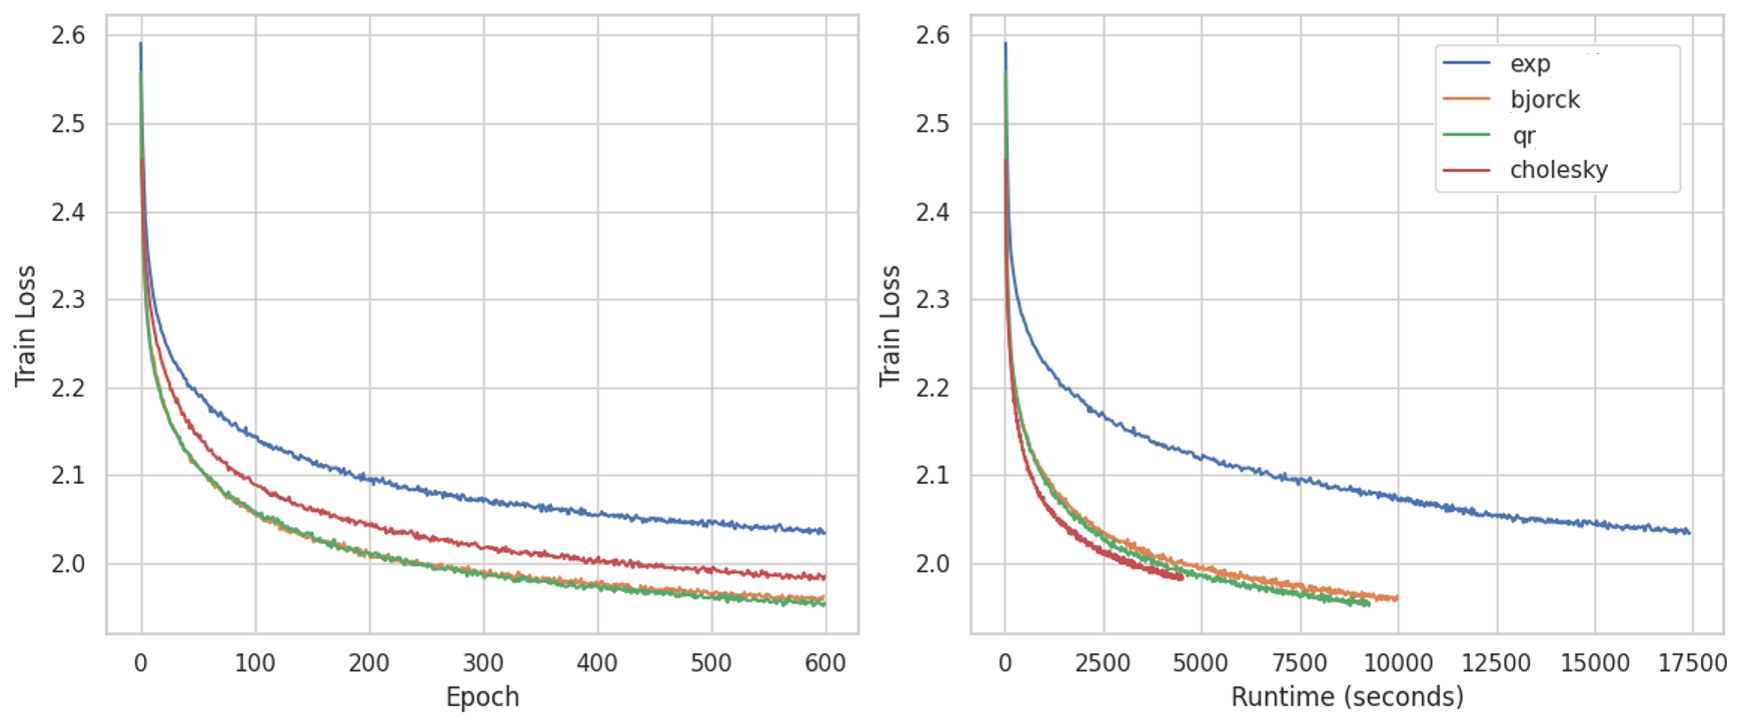
\includegraphics[width=0.9\textwidth]{flash_bcop/figs/ortho_bench/orth_methods.png}
        \caption{Impact of the orthogonalization method on AOC: in the same setup as \cite{li_preventing_2019} we observe that the orthogonalization precedure can have a significant impact on the training time and training accuracy. Except from exponential method which suffers from limitations due to our way to handle non-square matrices, other methods shows similar performance given the same computation time.}
        \label{fig:ortho_bench}
    \end{figure*}

    Given these observations, we sticked to the original choice of Björck and Bowie algorithm, as it is GPU and mixed precision compliant. Thanks to our unit-testing scheme, we observed that once the matrix is constrained to be 1-Lipschitz, we can set $\beta=0.5$ (the maximum value for which convergence can be guaranteed). This allows us to lower the number of iterations to 12 without affecting orthogonality.

\section{Empirical evaluation of the Lipschitz constant of our method} \label{ap:unit_testing}

    \paragraph{Evaluating the Lipschitz constant of a network}
    Beyond the creation of a constrained layer, the evaluation of the Lipschitz constant of a layer is by itself an active field: early work used fast Fourier transform to evaluate a lower bound of the Lipschitz constant of a convolutional layer with circular padding \cite{sedghi_singular_2019}. This work was later improved with a method that is quicker \cite{senderovich_towards_2022}, supports other types of padding \cite{grishina_tight_2024}, or allows the extraction of a larger part of the spectrum \cite{boroojeny_spectrum_2024}. The work of \cite{delattre2023efficient} \cite{delattre2024spectral} allows us to compute a certifiable upper bound efficiently under different types of padding.
    It is worth recalling that inferring the global Lipschitz constant of a network given the Lipschitz constant of each layer is an NP-Hard problem\cite{virmaux2018lipschitz}. Then, \cite{pauli_lipschitz_2024,fazlyab_efficient_2019,wang2024scalability} aim to tackle using SDP (Semi-definite programming) tools. Our work can also contribute to this issue as the orthogonal layer allows a tighter product bound (ie. bound using the product of the Lipschitz constant of each layer to evaluate the constant of the whole network).

    \paragraph{The need for an empirical evaluation of the Lipschitz constant of AOC.}

    Despite the theoretical guarantees ensuring orthogonality in our construction, empirical checks are necessary to confirm implementation correctness. Such verification prevents two types of issues:
    \begin{enumerate}
        \item \textbf{Checking of numerical instabilities:} Issues arising from floating-point precision, such as those introduced by small epsilon values added to avoid division by zero.
        \item \textbf{Checking for implementation discrepancies:} Differences between mathematical formalism and its translation to popular frameworks (e.g., SOC proofs assume circular padding, while its implementation uses zero padding).
    \end{enumerate}

    % Alongside the proofs that ensure that our construction is orthogonal, we must check that our implementation is correct. The two main sources of errors are often: 
    % \begin{enumerate}
    %     \item Numerical issues that might exploit floating point precision. A prime example is the computation of an inverse with an epsilon to avoid division by zero.
    %     \item Discrepancies between the mathematical formalism and its implementation in popular frameworks. For instance, proofs done in the frequency domain assume circular padding, while code implementations in popular frameworks assume zero padding by default.
    % \end{enumerate}  

% \paragraph{Methods for Evaluation}

% To ensure robustness, we employed two distinct methods:
% \begin{enumerate}
%     \item \textbf{Explicit SVD on Toeplitz Matrices:} Using the impulse response approach, we construct the Toeplitz matrix for any padding and stride, allowing direct computation of singular values. This method, though accurate, is computationally expensive for large input images.
%     \item \textbf{Product Bound for BCOP and RKO Kernels:} The upper bound for the BCOP kernel is computed using standard methods, while the SVD of the reshaped RKO kernel is used for direct evaluation. The smallest singular value is derived via $\sigma_{\text{min}}(K) = \sigma_{\text{max}} - \sigma_{\text{max}}(\sigma_{\text{max}}I - K)$. This approach is exact when $\sigma_{\text{min}} = \sigma_{\text{max}} = 1$ and is suitable for scalable unit testing.
% \end{enumerate}

% \paragraph{Unit Testing for Implementation Validation}

% We applied both methods in unit tests to verify orthogonality and correctness. The tests targeted the following sources of error:
% \begin{itemize}
%     \item Numerical instabilities from floating-point operations.
%     \item Padding mismatches between theoretical proofs and practical implementations.
% \end{itemize}

% Additionally, we leveraged the orthogonality property for practical verification. For example:
% \begin{equation}
%     (S_s K)(S_s K)^T = I \quad \text{(row orthogonal)}
% \end{equation}
% This can be verified by composing a strided orthogonal convolution followed by its transposed counterpart.

% \paragraph{Key Observations}

% \begin{itemize}
%     \item Tests were conducted for various kernel sizes, strides, dilations, input/output channels, and padding configurations. Each configuration was evaluated using both methods.
%     \item Small 8x8 images were utilized for explicit Toeplitz construction to identify padding-related issues. A tolerance of $10^{-4}$ was maintained for singular value checks.
%     \item All branches of our optimization tree (Fig. 2c in the main paper) were tested independently, confirming compatibility across parameter combinations.
% \end{itemize}

% In total, 1442 test cases were executed, divided as follows:
% \begin{itemize}
%     \item Block Convolution: 640 tests
%     \item Standard Convolution: 418 tests (72 common CNN configurations, 150 for extended strides configurations, 24 for even kernel sizes, 24 for depthwise configurations, 100 for case where stride equals kernel size)
%     \item Transposed Convolution: 384 tests
%     \item RKO: 370 tests
% \end{itemize}

% These tests demonstrate the correctness and scalability of our implementation under diverse configurations, ensuring robust layer construction for practical deployment.

    \paragraph{Checking the orthogonality of a layer under stride, group, transposition, and dilation conditions.}
    The numerical stability and the convergence of an orthogonal layer is dependent on the training hyper-parameters: mainly the number of iterations used in most methods, but the learning rate and weight decay can also play a significant role. We then need an evaluation method that scales along with the convolution and that can be used at the end of each training. On the other hand, as scalable methods can be imperfect, we also need a method that computes very precise bounds without making any assumptions on the layer parameters (like padding, or stride). In order to overcome this, we tested our layers with two distinct methods:
    \begin{enumerate}
        \item  \textbf{Explicit SVD on Toeplitz Matrices:} Using the impulse response approach, we construct the Toeplitz matrix for any padding and stride, allowing direct computation of singular values. This method, though accurate, is computationally expensive for large input images. \todo{Talk about Delattre 2024 and Delattre 2023}
        \item \textbf{Product Bound for BCOP and RKO Kernels:} The upper bound for the BCOP kernel is computed using standard methods, while the SVD of the reshaped RKO kernel is used for direct evaluation.
        % \item Separate computation of min/max singular value of both the BCOP and RKO kernel. Usual methods can be applied to compute the upper bound of the BCOP kernel, while the SVD can be directly applied to the reshaped kernel from RKO. The smallest singular value can be computed with the same algorithm as $\sigma_{min}(\kernel{K}) = \sigma_{max} - \sigma_{max}(\sigma_{max} \kernelid - \kernel{K}) $ \thib{todo clean this}. While this approach uses the product bound, this method is exact if $\sigma_{min} = \sigma_{max} = 1$. This makes this approach suitable for unit testing and sanity checking of layers at scale.
    \end{enumerate}

    \paragraph{Unit testing of the implementation.} We used both of these two approaches in our unit tests. This enables us to ensure that the second method (which is faster and more scalable) is correct to check that our layer is effectively orthogonal. Also, our layer unlocks the use of the transposed convolution, which can be used to compute directly the equation of orthogonal layers:
    \begin{align*}
        (\toepstride{s} \toep{K})(\toepstride{s} \toep{K})^T &= \toepid \quad \text{(row orthogonal)} \\
        \convcode{\kernel{K}}{\convtrcode{\kernel{K}}{x}{s}}{s} &= x
    \end{align*}
    Naturally, the other direction can also be verified for column orthogonal layers.

    To follow the optimization depicted in \cref{fig:method_simplify}, we tested each branch independently. For each branch, we tested multiple values for kernel size, stride, dilation, input channels, and output channels. For the kernel size, along with standard configurations of $3 \times 3$ and $5 \times 5$ kernels, we also covered cases for $1 \times 1$ kernels and even-sized kernels. For input/output channels, we covered various values and all the inequalities discussed in this paper (for instance when $c_o > c_is^2$).
    We ran similar tests for transposed convolution. As the computation of the singular values using the explicit construction of the Toeplitz matrix is quite expensive, we used it on small $8 \times 8$ images, this is also a good way to check for padding issues, as the kernel size is not negligible with respect to the image size. All the checks over the singular values for both methods were done with a tolerance of $1e^{-4}$. 

    Finally, we tested independently the properties of the \Bconv{} and the batched \Bconv{}.

    This amounts to 1442 tests that have the following repartition:
    \begin{itemize}
        \item block convolution: 640 tests
        \item convolution: 418 tests
        \begin{itemize}
            \item common configurations in CNN: 72 tests
            \item extended strided configurations: 150 tests
            \item even kernel size: 24 tests
            \item depthwise: 24 tests
            \item kernel size = stride : 100 tests
        \end{itemize}
        \item conv transpose: 384 tests
        \item RKO: 370 tests
    \end{itemize}

    This test bank was of precious use to confirm that all parameters can be combined together in practice. The total coverage of the library is 93\%.


\section{Using the content of this paper to improve SLL, SOC, and Sandwich}\label{sec:ap_improving_existing}

    In this section, we will explore how the content of this paper can be used to improve existing layers from the state of the art. %For SOC, we used the properties of the bloc convolution to improve the
    
    \subsection{Improving skew orthogonal convolution (SOC)} This method, introduced by \cite{singla_improved_2022} uses the fact that an exponential of a skew-symmetric matrix is orthogonal. The initial implementation builds a skew-symmetric kernel and computes the exponential convolution. However, without proper tools to compute the exponential of a convolution kernel, this exponential was computed implicitly for each input by using the Taylor expansion of the exponential (see \cref{eq:soc_implicit}).

        \begin{theorem}[Explicit conv exponential]

            We can use \cref{def_blocker} to compute explicitly the exponential of a kernel $\kernel{K}$:

            \begin{align}
                & x + \frac{\kernel{K}*x}{1!} + \frac{\kernel{K}*\kernel{K}*x}{2!} + \dots \label{eq:soc_implicit} \\
                = & \left(Id + \kernel{K} + \frac{\kernel{K} \mathbconv \kernel{K}}{2!} + \frac{\kernel{K} \mathbconv \kernel{K} \mathbconv \kernel{K} }{3!} + \dots \right) * x \label{eq:soc_explicit}            
            \end{align}
        \end{theorem}

         \Cref{eq:soc_explicit} shows that we can compute the exponential of a convolution kernel a single time, while the formulation in \cref{eq:soc_implicit} needs to be done for each input $x$. In other words, we can apply one conv instead of $n_{iter}$ convs. Note that the resulting kernel is then larger than the original one (as stated in  \cref{tab:big_picture}). In theory, this could unlock large speedups, but the gain is limited in practice as the implementation of convolution layers is optimized for small kernels and large images \cite{ding_scaling_2022}. However, the original implementation requires the storage of $n_{iter}$ maps, whereas our implementation only one. This, in practice, unlocks larger networks and batch sizes.

        Also, it is possible to handle a change in the number of channels and striding using a similar approach as AOC layers.

    \subsection{Improving SDP-based Lipschitz Layers (SLL)}
        % \begin{wrapfigure}{r}{0.65\textwidth}
    \begin{figure}[h]
        \centering
        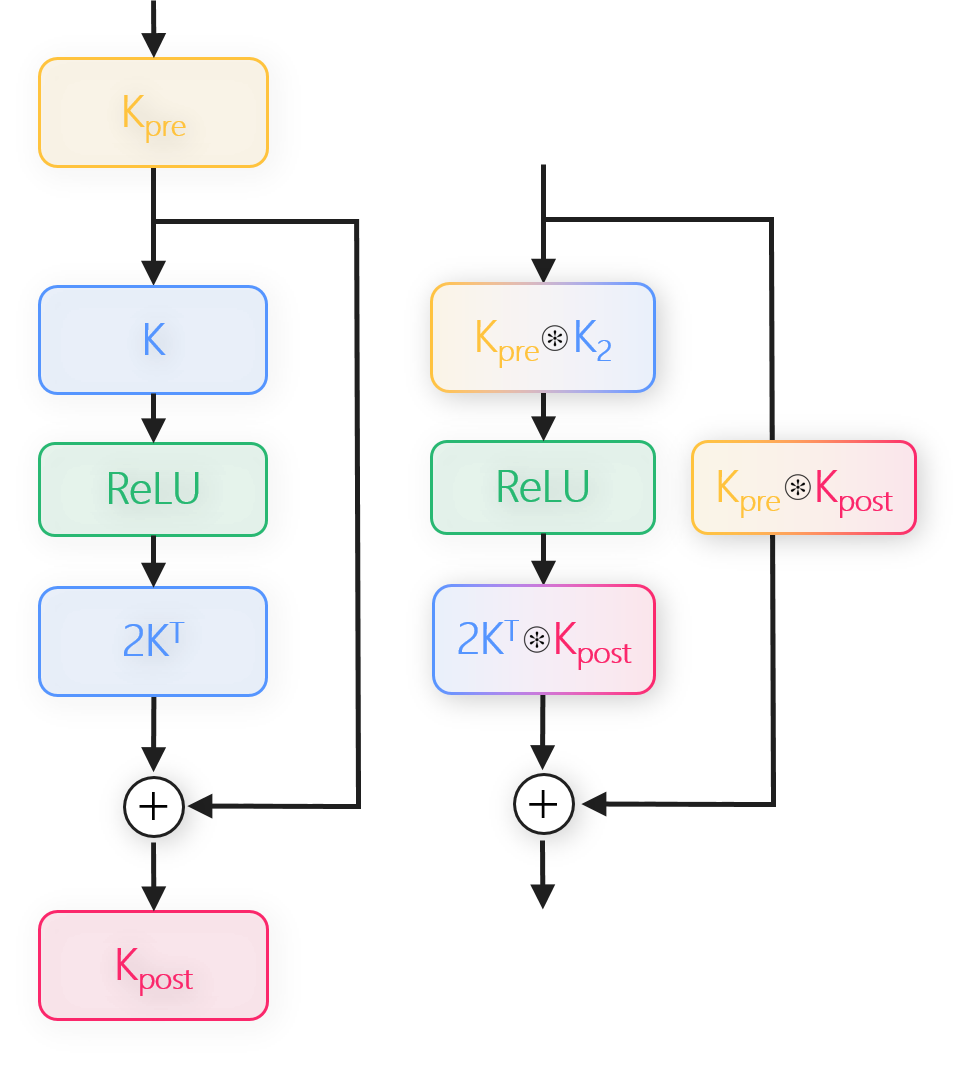
\includegraphics[width=0.45\linewidth]{flash_bcop/figs/illustrations/SLL_3.png}
        \caption{\textbf{The $\mathbconv$ can be used to enable $s\neq 1$ and $c_i \neq c_o$ configurations on SLL.} The flexibility of the $\mathbconv$ allows for operations resulting in a block with a similar structure as the original ResNet block.}
        \label{fig:SLL}
    \end{figure}

    SLL layer for convolutions, proposed in \cite{araujo_unified_2023}, is a 1-Lipschitz layer defined as:
    \[
        y = x - 2\kernel{K}^T \convker{} ( \sigma ( \kernel{K} \convker{} x + b ))
    \]
    Note that in the original paper, the equation is noted with product of two matrices $WT^{-\frac{1}{2}}$, for convolutions it represents toeplitz matrix, i.e. $WT^{-\frac{1}{2}} =  \toep{K}$.
    
    SLL layer does not natively support neither strides nor changes in the channel size.
    We propose to use the $\mathbconv$ to derive a block, based on SLL, that supports stride and $c_i \neq c_o$, and can replace the strided convolutions of the residual branch in architectures like ResNet.  
    
    A natural first step is to append a strided convolution after a SLL block. This layer, $conv_{K_{post}}\circ SLL$, can then be fused in the SLL block thanks to  \cref{prop:bilinear}:
    \begin{align*}
        y =& \kernel{K}_{post} \convker{s} (x - 2\kernel{K}^T \convker{} ( \sigma ( \kernel{K} \convker{} x + b ))) \\
        =&  \kernel{K}_{post} \convker{s} x - 2(\kernel{K}_{post} \mathbconv \kernel{K}^T) \convker{s} ( \sigma ( \kernel{K} \convker{} x + b ))) \\
    \end{align*}
    This allows to build a block based on SLL and that supports stride and channel changes. However, this creates an asymmetry between the convolution before the activation and the one after the activation (that has a larger kernel size). 
    
    We propose also to add a second convolution before the SLL block, $conv_{K_{post}}\circ SLL\circ conv_{K_{pre}}$allowing better control over the kernel size of each convolution:
    \begin{align*}
        y = &\kernel{K}_{post} \convker{s} \kernel{K}_{pre} \convker{} x \\
        & - 2(\kernel{K}_{post} \mathbconv \kernel{K}^T) \convker{s} ( \sigma ( \kernel{K} \convker{} \kernel{K}_{pre} \convker{} x + b ))) \\
        = &(\kernel{K}_{post} \mathbconv \kernel{K}_{pre}) \convker{s} x \\
        & - 2(\kernel{K}_{post} \mathbconv \kernel{K}^T) \convker{s} ( \sigma ( (\kernel{K} \mathbconv \kernel{K}_{pre}) \convker{} x + b ))) \\
    \end{align*}
    
    The proposed block is still a 1-Lipschitz layer (as a composition of 1-Lipschitz and orthogonal layers), and support efficiently strides and changes of kernel sizes.
    A visual description is provided in \cref{fig:SLL}. This approach is more efficient than the explicit construction that uses 3 distinct convolutions, as kernels are merged once per batch, and intermediate activations of extra convolutions do not need to be stored backward. Typically, when $\kernel{K}$, $\kernel{K}_{pre}$ and $\kernel{K}_{post}$ are $2 \times 2$ convolutions, this results in a residual block with two $3 \times 3$ convolutions in one branch and a single $4 \times 4$ convolution (with stride 2) in the second. This is very similar to transition blocks found in typical residual networks.

    % \paragraph{Improving Cayley\cite{trockman_orthogonalizing_2021}:} Cayley is a method that performs its orthgonalisation in the frequency domain using FFT. Hence our approach cannot be directly used to handle stride or changes in number of channels. However, by using \cref{def:orthogonal}, a change in the number of channel can be handle a-priori by dropping a part of the orthgonal weight matrix. Also the optimizations described in \cref{sec:implem} can be applied to handle striding (striding must be performed directly in Fourier domain in order to be efficient).

    % \paragraph{Improving sandwich layers.} This approach aims to construct a 1-Lipschitz network globally rather than constraining each layer independently. In practice, this can be done either by I) adding constraints between layers or ii) creating layers that contain a non-linearity inside (a.k.a sandwich layers). However, sandwich layers requires an orthogonal matrix at its core. For convolutional layers, this is done by performing the orthogonalization of the layer in the Fourier domain (method from \cite{trockman_orthogonalizing_2021}) as shown in their algorithm 1:
    \subsection{Improving Sandwich Layers}
    Introduced by \cite{wang_direct_2023}, this approach aims to construct a 1-Lipschitz network globally rather than constraining each layer independently. In practice, this can be done either by (i) adding constraints between layers or (ii) creating layers that incorporate a non-linearity internally (a.k.a. sandwich layers). However, sandwich layers require an orthogonal matrix at their core. For convolutional layers, this is achieved by performing the orthogonalization of the layer in the Fourier domain, as described in the method from \cite{trockman_orthogonalizing_2021} and shown in their Algorithm 1.
    \begin{algorithm}
        \caption{Sandwich convolutional layer (from \cite{wang_direct_2023})}
        \begin{algorithmic}[1]
            \Require $h_\text{in} \in \mathbb{R}^{p \times s \times s}$, $P \in \mathbb{R}^{(p+q) \times q \times s \times s}$, $d \in \mathbb{R}^q$
            \State $\hat{h}_\text{in} \gets \text{FFT}(h_\text{in})$
            \State $\Psi \gets \text{diag}(e^d), \, \begin{bmatrix} \tilde{A} & \tilde{B} \end{bmatrix}^* \gets \text{Cayley}(\text{FFT}(P))$
            \State $\hat{h}[:, i, j] \gets \sqrt{2} \tilde{B}[:, :, i, j] \hat{h}_\text{in}[:, i, j]$
            \State $\hat{h} \gets \text{FFT}(\sigma(\text{FFT}^{-1}(\hat{h}) + b))$
            \State $\hat{h}_\text{out}[:, i, j] \gets \sqrt{2} \tilde{A}[:, :, i, j] \Psi \hat{h}[:, i, j]$
            \State $h_\text{out} \gets \text{FFT}^{-1}(\hat{h}_\text{out})$
        \end{algorithmic}
    \end{algorithm}

    We can leverage AOC to construct the kernel of an orthogonal convolution, replacing the expensive operation performed in the Fourier domain. Thus, we can construct two kernels, $\kernel{A}$ and $\kernel{B}$, with appropriate constraints between the two and apply the rescaling and non-linearity directly in pixel space:
    % We can leverage AOC to construct the kernel of an orthogonal convolution, replacing the expensive operation done in the Fourier domain. We can hence construct two kernels $\kernel{A}$ and $\kernel{B}$ with appropriate constraints and apply the rescaling and non-linearity directly in pixel space:
    \[
    h_\text{out} = \sqrt{2} \kernel{A}^\top \convker{} \Psi \sigma \left( \sqrt{2} \Psi^{-1} \kernel{B} \convker{} h_\text{in} + b \right)
    \]
    The use of the Fourier transform is costly for two reasons: first, it necessitates computation with complex values; and second, the cost of the operation depends on the input size, which can be prohibitive in large-scale settings with $224 \times 224$ images. Consequently, our approach can make such a layer more scalable.
    % The use of the Fourier transform is costly for two reasons: first, it forces computation with complex values, and second, the cost of the operation depends on the input size which can be prohibitive in large-scale settings with $224\times 224$ images. Hence our approach can make such a layer more scalable.

    % \paragraph{Improving other methods} beyond the aforementioned methods that can benefit non-trivial improvements, we can leverage our approach to improve many other orthogonal convolutional layers. We can notice that the BCOP component can be replaced by a given orthogonal layer, resulting in native striding on those layers. Similarly we can allow for groups, trnasposed convolution and dilation.

    \subsection{Extending Applicability to other methods.} Beyond the previously discussed approaches that show meaningful opportunities for improvement, our method can enhance a wide range of orthogonal convolutional layers. Specifically, we can incorporate our framework into any alternative orthogonal layers, enabling native support for strides in those layers. Furthermore, our approach can unlock features such as grouped convolutions, transposed convolutions, and dilations, broadening its utility and adaptability.

% \section{Convolutional arithmetic, a tutorial} \label{sec:ap_math}

    % We will consider convolutional layers characterized by $c_o$, the number of output channels, $c_i$ the number of input channels, $k$ the size of the kernel, $s$ the stride parameter and $g$ the number of groups. For the sake of readability we the notations focus on the case of square kernels with $g=1$ (all proofs holds for non square kernel and other values for $g$). We consider convolution with circular padding\footnote{ extension to other type of padding will be discussed later}. The kernel tensor of the convolution is noted $\kernel{ K}\in\KbfS$ while $x\in\RR^{c_i\times h \times w}$ denote the input tensor. We can then describe the convolution operation with 3 different notations:
    % % Given an input $x\in\RR^{c_i\times h \times w}$, we note equivalently $\cKbf(x)=\Kbf\star x\in\RR^{c_o\frac{h}{2}\frac{w}{2}}$ the results of the application of the convolution of kernel $\Kbf$ on $x$.
    % \begin{align}
    %     y = \kernel{K} \convker{s} x & \quad  \text{(kernel notation)} \label{def_convker_app}\\
    %     \toepvec{y} = \toepstride{s} \toep{K}\toepvec{x} & \quad  \text{(Toeplitz notation)} \label{def_convtoep_app} \\
    %     y = \convcode{K}{x}{s} &  \quad \text{(code notation)} \label{def_convcode_app}
    % \end{align}

    %  \Cref{def_convker} defines the convolution operation with kernel $ \kernel{K}$ and stride $s$ applied on $x$.  \Cref{def_convtoep} highlight that this convolution operation is equivalent to a linear application defined by the matrix product between a Toeplitz matrix $ \toep{K} \in \KkS $ and a vector $ \toepvec{x} \in \RR^{c_ihw} $ which is obtained by flattening $x$. The striding operation is noted by a masking matrix $\toepstride{s} \in \RR^{c_o\frac{h}{s}\frac{w}{s} \times c_ohw}$ with ones on the selected entries and zeros elsewhere. When $s=1$, we have $\toepstride{1} = \toepid$ the identity matrix (whose kernel is denoted $ \kernelid$).  \Cref{def_convcode} shows that these notations can be conveniently converted into pseudo code.
    
    % % We denote $\Kk\in\KkS$ the equivalent toeplitz matrix that implement the application of the convolution on a vectorized input $\Vect(x)\in\RR^{c_is^2\frac{h}{2}\frac{w}{2}}$: 
    % % \[
    % % \Kk\Vect(x) = \Vect(\Kbf\convker x)\in\RR^{c_o\frac{h}{2}\frac{w}{2}}
    % % \]
    % % We will note by extension $\Kbf^T$ the kernel corresponding to the transpose convolution $\Kk^T$.

    % \begin{definition}[transposed convolution] transposed convolution can be defined as following:
    %     \begin{align}
    %         y = \kernel{K}^T \convker{\frac{1}{s}} x \label{def_transposeker}\\
    %         \toepvec{y} = (\toepstride{s} \toep{K})^T\toepvec{x} = \toep{K}^T \toepstride{s}^T \toepvec{x} \label{def_transposetoep} \\
    %         y = \convtrcode{K}{x}{s} \label{def_transposecode}
    %     \end{align}
    %     Which correspond to the transposition of the underlying Toeplitz matrix ( \cref{def_transposetoep}). This can be defined as the standard convolution with transposed kernel and fractional striding ( \cref{def_transposeker}). $ \kernel{K}^T \in \RR^{c_i \times c_o \times k \times k } $ is obtained by transposing the two firsts dimensions and reversing the two last dimensions. The kernel is not transposed in  \cref{def_transposecode} to match the implementation of the transposed convolution found in pytorch.
    % \end{definition}

    % \begin{definition}[\Bconv{} $\mathbconv$] The bloc convolution allows to fuse two convolutions by computing the equivalent kernel without explicitly computing the two convolutions: 
    %     \begin{align}
    %         (\kernel{B} \mathbconv \kernel{A}) \convker{s} x = \kernel{B} \convker{s} (\kernel{A} \convker{1} x ) \label{def_blocker}\\
    %         \toepstride{s} (\toep{B} \toep{A}) \toepvec{x} = (\toepstride{s} \toep{B}) \toep{A} \toepvec{x} \label{def_bloctoep} \\
    %         \shortconvcode{A \mathbconv B}{x}{s} = \shortconvcode{B}{\shortconvcode{A}{x}{1}}{s} \label{def_bloccode}
    %     \end{align}
    %     This operator is defined assuming the number of input channels of the second convolution matches the number of input channels of the second convolution. Given $ \kernel{A} \in \RR^{c_{int}\times c_i \times k_1 \times k_1 } $ and $ \kernel{B} \in \RR^{c_{o}\times c_{int} \times k_2 \times k_2 } $ then $ \kernel{B} \mathbconv \kernel{A} \in \RR^{c_o \times c_i \times k_1 + k_2 - 1 \times k_1 + k_2 - 1 } $.
    % \end{definition}

    
    % \textbf{Associativity}: The  $\mathbconv$  operation is associative (given the kernel are compatible $\compat{A}{B}$,$\compat{B}{C}$): 
    %     \[ A \mathbconv (B \mathbconv C) = (A \mathbconv B ) \mathbconv C \]
    
    % \textbf{Bilinearity}: Given two convolutions $A$ and $B$ with the same channel size, a third convolution $C$ compatible with $A$ and $B$ ($\compat{A}{C}$,$\compat{B}{C}$),and two scalars $\lambda_1,\lambda_2\in\RR$: \red{ca fait bcp d'hypotheses ca ira surement en annexe}
    %     \[ (\lambda_1 A + \lambda_2 B) \mathbconv C = \lambda_1 A \mathbconv C +  \lambda_2 B \mathbconv C 
    %     \]

    % \textbf{Non commutativity}: the \Bconv{} is not commutative, since in general the composition of convolution is not.
    % %nvolution \red{(since composition of convolution is not)}:
    % \[ A \mathbconv B \neq B \mathbconv A \]
    % %It is a linear application:
    % %\[ \lambda_1 A * x + \lambda_2 B * x = (\lambda_1 A + \lambda_2 B) * x \]


\section{About the incomplete parametrization of BCOP and SC-fac} \label{sec:ap_incomplete}


    As mentioned earlier, both BCOP and SC-Fac exhibit an incomplete parametrization. BCOP has an incomplete parametrization for 2D convolutions, while SC-Fac offers a complete parametrization but only for separable convolutions.
    
    \subsection{Understanding the Limitations of BCOP}
    The limitations of BCOP parametrization have significant implications for its use in practical applications. Below, we provide a detailed discussion of the known limitations:
    
    \begin{itemize}
        \item The authors presented a counterexample involving a $2\times 2$ convolution that is orthogonal but cannot be parametrized by BCOP. This highlights the incomplete nature of BCOP for parametrizing certain convolutional layers.
        \item However, this counterexample can be parametrized by a $3\times 3$ BCOP convolution, which suggests that increasing the kernel size can potentially address the issue of incomplete parametrization.
        \item This does not imply that all $2\times 2$ orthogonal convolutions can be parametrized using $3\times 3$ BCOP convolutions, but it provides a useful starting point. It indicates that while BCOP may struggle with certain cases at smaller kernel sizes, increasing the kernel size could offer a pathway to improve coverage.
    \end{itemize}
    
    This problem is more complex than initially expected: the parametrization space of BCOP is disconnected. In simple terms, the disconnected nature of the parametrization space means that certain transformations cannot be continuously reached from others within the same parametrization framework. Nevertheless, a BCOP convolution with $c$ channels can have a connected component that represents all convolutions with $c/2$ channels. This property indicates that, although BCOP may not cover the entire space of orthogonal convolutions, it has subsets that can be effectively utilized for lower-dimensional problems.
    
    Another noteworthy point is that the disconnected nature of the parametrization space could limit the efficiency of optimization algorithms that rely on continuous transformations during training. In practice, this means that certain optimal configurations may not be reachable through gradient-based methods, which could hinder the overall performance of models employing BCOP convolutions.
    
    The issue of incomplete parametrization can be mitigated by increasing the number of channels and kernel size, highlighting the need for a scalable approach to address the challenge effectively. Increasing the number of channels provides more degrees of freedom, which may help cover more of the orthogonal convolution space while increasing the kernel size expands the range of spatial features that can be represented.\todo{add a remark about the idea of overparametrizations}

    Research on the complete parametrization of orthogonal convolutions with controlled kernel sizes remains an open question, AOC could benefit from further improvements in this area.
    % \subsection{Potential Solutions}
    % The root cause of the incompleteness lies in the fact that there exist $2 \times 2$ kernels that are not separable, while the composition of $1 \times 2$ and $2 \times 1$ kernels is by design separable (this does not imply that the composition of separable $2 \times 2$ kernels is separable). A first step to address the limitations of BCOP parametrization would consist in finding a way to parametrize all orthogonal $2 \times 2$ kernels. Then this would also require proving that any $k \times k$ convolution can be obtained by composing such $2 \times 2$ kernels. 
    
    % Ultimately, solving the issue of incomplete parametrization in BCOP requires a combination of theoretical advancements and practical strategies. Developing a deeper understanding of the parametrization space and exploring new mathematical formulations could provide a foundation for more effective solutions. In addition, practical methods such as increasing kernel size, employing hybrid approaches, and using regularization can help mitigate the limitations in existing applications.
    
    
        % \begin{figure*}[ht!]
        %     \centering
        %     \includegraphics[width=0.45\linewidth]{flash_bcop/figs/benchmark/bloc_conv_speed_k.png}
        %     \includegraphics[width=0.45\linewidth]{flash_bcop/figs/benchmark/bloc_conv_speed_cin.png}
        %     \caption{\textbf{Our bloc convolution implementation is an order of magnitude faster than the original implementation:} as expected the method scales better with kernel size (left), but it also showed drastic improvement with respect to the number of input channels (right, log scale).}
        %     \label{fig:bloc_conv_speedup}
        % \end{figure*}

\section{Proofs}\label{sec:ap_proofs}

    \todo{cf remarques du reviewer 1. Vérifier les typos, clarifier le flow, et rendra plus lisible}

    \subsection{Proof of the $\mathbconv$ property:}\label{sec:ap_proofs_mathbconv}
        \todo{The proof of the $\mathbconv$ property in Appendix E1 already appears in Refs [31] and [64]. What is the difference between the authors' proof and those in Refs [31] and [64]? If there are differences, it would be helpful to sketch what they are.}
        Although already shown in previous papers \cite{li_preventing_2019}, \cite{xiao_dynamical_2018}, we provide the proof in the 1D case to help the reader understand the mechanism of the $\mathbconv$ operator.
        Given a vector $x\in\RR^{c_{in}\times w}$, and two kernels $\kernel{A}\in\RR^{c_{int}\times c_i \times k_A}$ and $\kernel{B}\in\RR^{c_o\times c_{int} \times k_B}$. We suppose that $\kernel{A}$ is zero-padded, i.e., $\kernel{A}_{c,n,i} = 0$ if $i<0$ or $i\geq k_A$.
    \begin{proof}
    \begin{align*}
            y &= \kernel{A}\convker{}x,\text{such as,  } \\ 
            y_{c,j}&=\sum_{n = 0}^{c_i-1}\sum_{j' = 0}^{k_A-1}\kernel{A}_{c,n,j'}x_{n,j-j'}\\
    		z &= \kernel{B}\convker{}y=(\kernel{B}\mathbconv \kernel{A})\convker{}x,\text{such as,  }
    \end{align*}
    \begin{align*}
      z_{m,l}&=\sum_{c = 0}^{c_{int}-1}\sum_{i' = 0}^{k_B-1}\kernel{B}_{m,c,i'}y_{c,l-i'}\\
    		&=\sum_{c = 0}^{c_{int}-1}\sum_{i' = 0}^{k_B-1}\kernel{B}_{m,c,i'}\sum_{k = 0}^{c_i-1}\sum_{j' = 0}^{k_A-1}\kernel{A}_{c,k,j'}x_{k,l-i'-j'}\\
    		&= \sum_{k = 0}^{c_i-1}\sum_{j' = 0}^{k_A-1}\sum_{c = 0}^{c_{int}-1}\sum_{i' = 0}^{k_B-1}\kernel{B}_{m,c,i'}\kernel{A}_{c,k,j'}x_{k,l-i'-j'}\\
      &= \sum_{k = 0}^{c_i-1}\sum_{l' = 0}^{k_A+k_B-1}\sum_{c = 0}^{c_{int}-1}\sum_{i' = 0}^{k_B-1}\kernel{B}_{m,c,i'}\kernel{A}_{c,k,l'-i'}x_{k,l-l'}   &\quad (\text{with } l'=i'+j')\\
    		&= \sum_{k = 0}^{c_i-1}\sum_{l' = 0}^{k_A+k_B-1}{(\kernel{B}\mathbconv \kernel{A})}_{m,k,l'}x_{k,l-l'}   &\quad (\text{direct formulation of } (\kernel{B}\mathbconv \kernel{A})\convker{}x)
    \end{align*}
      with thus
      \[
      {(\kernel{B}\mathbconv \kernel{A})}_{m,n,i} = \sum_{c = 0}^{c_{int}-1}\sum_{i' = 0}^{k_B-1} \kernel{B}_{m,c,i'} . \kernel{A}_{c,n,i-i'}
      \]
\end{proof}


    \subsection{Recall of $\mathbconv$ other properties}
Two kernels $\kernel{A}$ and $\kernel{B}$ are said compatible for the $\kernel{B}\mathbconv\kernel{A}$ operation when the number of input channels of the second convolution $\kernel{B}$ matches the number of output channels of the first convolution. This condition is denoted as $\compat{A}{B}$.

We present here several properties of the  \Bconv{} operator  $\mathbconv$: 
    
        \begin{proposition}[Associativity]\label{prop:associativity} The $\mathbconv$ operation is associative (given compatible kernels $\compat{A}{B}$ and $\compat{B}{C}$): 
            \[ A \mathbconv (B \mathbconv C) = (A \mathbconv B) \mathbconv C \]
            
        \end{proposition}
        
        \begin{proposition}[Bi-linearity]\label{prop:bilinear} Given two convolutions $A$ and $B$ with the same channel sizes, a third convolution $C$ compatible with $A$ and $B$ ($\compat{A}{C}$, $\compat{B}{C}$), and two scalars $\lambda_1, \lambda_2 \in \RR$:
            \[ (\lambda_1 A + \lambda_2 B) \mathbconv C = \lambda_1 A \mathbconv C +  \lambda_2 B \mathbconv C 
            \]
        \end{proposition}
        
        \begin{proposition}[Non-Commutativity] Even when $\compat{A}{B}$ and $\compat{B}{A}$ hold, \Bconv{} is not commutative, as convolution composition is generally not commutative:
        \[
            \toep{A} \toep{B} \neq \toep{B} \toep{A} \implies \kernel{A} \mathbconv \kernel{B} \neq \kernel{B} \mathbconv \kernel{A} 
        \]
        \end{proposition}

    \subsection{Proof of the construction of $c\times c \times 1 \times 2$ orthogonal convolution}\label{sec:ap_1x2_ortho}

        This proof was already presented in \cite{li_preventing_2019}, but we include it here for the sake of completeness. %Given the construction explained in  \cref{sec:AOC}, we can show that 
        Given a symmetric orthogonal projectors $N\in\RR^{c\times c}$  such as:
        \[
            N = N^2 = N^T \quad \text{and} \quad (I - N) = (I - N)^2 = (I - N)^T
        \]
        Considering $N$ and $I-N$ as $\RR^{c\times c\times 1\times 1}$ convolution kernels, 
        we can build a  convolution kernel  $\kernel{P}\in\RR^{c\times c\times 1\times 2}$  by: 
        \[
        \kernel{P} = \mathtt{stack(}[\kernel{N}, \kernel{I - N}]\mathtt{, axis=-1)}        
        \]
        %\Rightarrow \kernel{P} \mathbconv \kernel{P}^T = \kernel{I}  
        For readability, we will write $\kernel{P} = \left[ N , I-N \right]$ as a compact notation for the stacked kernels. We will prove that such a kernel $\kernel{P}$ defines an  orthogonal convolution. Since this convolution has no stride $s=1$, as stated in  \cref{sec:construction}, this is equivalent to :
        \[
        \kernel{P} \mathbconv \kernel{P}^T = \kernel{P}^T \mathbconv \kernel{P} = \kernel{I} 
        \]
        %:
        %\[
        %    \kernel{P} = \left[ N , I-N \right]
        %\]

    \begin{proof}

        %As we assume $s=1$, we can say that $\kernel{P}$ is orthogonal if $\kernel{P} \mathbconv \kernel{P}^T = \kernel{P}^T \mathbconv \kernel{P} = \kernelid $. 
        We can  compute explicitly the resulting kernel for $\kernel{P} \mathbconv \kernel{P}^T$:
        \begin{align*}
            & \kernel{P} \mathbconv \kernel{P}^T =\\
            & = \left[ N , I-N \right] \mathbconv \left[ (I-N)^T , N^T \right] \\
            & = \left[ N(I-N)^T , NN^T + (I-N)(I-N)^T, (I-N)N^T  \right] \\
            & = \left[ N(I-N) , N^2 + (I-N)(I-N), (I-N)N  \right] \\
            & = \left[ N-N^2 , N^2 + I - 2N + N^2, N-N^2  \right] \\
            & = \left[ N-N , N + I - 2N + 2N^2, N-N  \right] \\
            & = \left[ 0, I, 0  \right] \\
        \end{align*}
    \end{proof}

        The third line is the matrix application of the $\mathbconv$  with two $1\times 2$ kernels (\cref{eq:blockconv}). The following lines are based on the trivial application of the symmetric projector property.

        \paragraph{Construction of symmetric projectors.} \todo{maybe move this into a larger part dedicated to implementation details} Following the construction described in \cite{li_preventing_2019} a symmetric projectors $N \in \RR^{c\times c}$ can be constructed based a column-orthogonal matrix $N_0 \in \RR^{c\times \frac{c}{2}}$:
        \begin{align*}
            \text{given }& N_0 \in \RR^{c\times \frac{c}{2}} \text{, such that }  N_0^T N_0 = I 
            %\\
            %N = N_0 N_0^T  &\implies N = N^T = N^2 \\
            %&\implies (I-N) = (I-N)^T = (I-N)^2
        \end{align*}
        The matrices $N = N_0 N_0^T$ and $I-N$ are a symmetric projectors.

    \begin{proof}
        This proof was already presented in \cite{li_preventing_2019}, but we include it here for the sake of completeness.
        \begin{align*}
        N^2 &=(N_0 N_0^T)(N_0 N_0^T) \\
        &= N_0(N_0^TN_0)N_0^T \\
        &= N_0N_0^T\\
        &=N=N^T
        \end{align*}
        
        \begin{align*}
        (I-N)^2 &=(I-N_0 N_0^T)(I-N_0 N_0^T) \\
        &= I -2N_0N_0^T + (N_0N_0^T)(N_0N_0^T) \\
        &= I-N_0N_0^T\\
        &=I-N=(I-N)^T
        \end{align*}
    \end{proof}

    \subsection{RKO kernel with stride \texorpdfstring{$s=k$}{s=k} builds an orthogonal convolution}\label{sec:ap_proof_rko}
    %is orthogonal when $k=s$}
    The RKO method considers a convolution $\shortconvcode{K}{.}{s}$ with a kernel $\kernel{K}\in\RR^{c_o\times c_i\times k\times k}$, built by reshaping an orthogonal matrix $K'\in\RR^{c_o\times c_i.k^2}$. The matrix $K'$ can be obtained for instance by  the Björck and Bowie orthogonalization scheme \cite{bjorck1971iterative} and verifies $K'K'^T=Id$ for row orthogonality (resp. $K'^TK'=Id$ for column) .
    
    In the general case, the resulting convolution is not orthogonal \cite{achour2023existencestabilityscalabilityorthogonal}. We prove that in the special case where the kernel and the stride are equal, the $\shortconvcode{K}{.}{k}$ with stride $s=k$  is orthogonal.

    
        \begin{proof}
        $\forall x\in\RR^{c_i\times h\times w}$, where we suppose that $h,w$ are multiple of $s$, we have:
        \begin{align*}
            \shortconvcode{K}{x}{k}_{h,i,j}            &= \sum_{c = 0}^{c_{i}-1} \sum_{i' = 0}^{k - 1} \sum_{j' = 0}^{k - 1} K_{h,c,i',j'}x_{c,ik-i',jk-j'} \\
            &=  \sum_{c = 0}^{c_{i}k^2-1} K'_{h,c}\bar{x}_{c,i,j} \\
            &= (K'\bar{x})_{h,i,j}
        \end{align*}
        where $\bar{x} \in\RR^{c_ik^2,\frac{h}{k},\frac{w}{k}}$ is defined by:
        \[
        \bar{x}_{.,i,j} = \begin{bmatrix}x_{0,ik,jk}\\x_{0,ik-1,jk}\\ \vdots \\ x_{0,(i-1)k+1,jk}\\ x_{0,ik,jk-1}\\ \vdots \\ x_{1,ik,jk}\\ \vdots \\ x_{c_i-1,(i-1)k+1,(j-1)k+1}\end{bmatrix} 
        \]
        Since there is no overlap between the receptive field of each output, $\bar{x}=Px$ where the matrix $P$ is a permutation (similar to an invertible downsampling with factor k), which is by definition orthogonal.

        In the case of row orthogonality for $K'$, we have:
\begin{align*}
    &\shortconvcode{K}{\convtrcode{K}{x}{k}}{k} \\
    &= K'P(K'P)^Tx \\
    &= K'PP^TK'^Tx  & \quad \text{(P is orthogonal)}\\ 
    &= K'K'^Tx & \quad \text{(K' is orthogonal)}\\
    &= x
\end{align*}

        \end{proof}
        \todo{\franck{DONE mais j'ai pas trouvé plus clair}The proof of the orthogonality of RKO in Appendix E3 is incomplete and informal. Since there is no page limit for the Appendix, it would be better to provide a full and formal proof of all theoretical results presented in the paper.}

        %The proof is given by the property that when $k=s$ the convolution can be decomposed into a reshaping operation (invertible downsampling with factor s) followed by a $1\times 1$ convolution with kernel $K'\in\RR^{c_o\times c_is^2 \times 1\times 1}$. The kernel $K'$ is the orthogonal matrix built by RKO method. 

    \subsection{AOC convolutions are orthogonal}
\label{sec:ap_proof_aoc_ortho}
        The construction of our method consists in composing a BCOP kernel $ \kernel{K}_{BCOP} \in \RRkernel{c}{c_i}{k-s}{k-s} $ followed by an RKO kernel $ \kernel{K}_{RKO} \in \RRkernel{c_o}{c}{s}{s} $. As we already proved that each kernel is orthogonal, we know that 
        \begin{align*}
            \toep{K}_{BCOP} \, \toep{K}_{BCOP}^T = \toepid \text{ when } c_i \geq c \\
            \toep{K}_{BCOP}^T \, \toep{K}_{BCOP} = \toepid \text{ when } c_i \leq c
        \end{align*}
        and that 
        \begin{align*}
            (\toepstride{s} \, \toep{K}_{RKO})(\toepstride{s} \, \toep{K}_{RKO})^T = \toepid \text{ when } c*s^2 \geq c_o \\
            (\toepstride{s} \, \toep{K}_{RKO})^T(\toepstride{s} \, \toep{K}_{RKO}) = \toepid \text{ when } c*s^2 \leq c_o
        \end{align*}
    We prove that with a correct choice of the internal dimension $c$, the strided AOC convolution with kernel $\kernel{K}_{AOC}= \kernel{K}_{\text{RKO}} \mathbconv \kernel{K}_{\text{BCOP}}$ is orthogonal.
    
        \begin{proof}
        As $c$ (the intermediate number of channels) is a free parameter we can demonstrate that our construction is orthogonal when  the convolutions are either both row orthogonal , or both column orthogonal (\cref{prop:composition_ortho}), i.e when:
        \begin{align*}
                              & c_i \geq c \text{  and  } c \geq \frac{c_o}{s^2} & \quad \text{(both row orthogonal)}\\
            \text{ or } \quad & c_i \leq c \text{  and  } c \leq \frac{c_o}{s^2} & \quad \text{(both column orthogonal)}
        \end{align*}
        In the first case, when $ c_i \geq \frac{c_o}{s^2}$The resulting convolution $(\toepstride{s} \, \toep{K}_{RKO} \, \toep{K}_{BCOP})$ is orthogonal for any $c$ such as  $ \frac{c_o}{s^2} \leq c \leq c_i$:
        \begin{align*}
            &(\toepstride{s} \, \toep{K}_{RKO} \, \toep{K}_{BCOP})(\toepstride{s} \, \toep{K}_{RKO} \, \toep{K}_{BCOP})^T \\
            = &(\toepstride{s} \, \toep{K}_{RKO})\toep{K}_{BCOP} \, \toep{K}_{BCOP}^T(\toepstride{s} \, \toep{K}_{RKO})^T & \quad (\toep{K}_{BCOP} \text{ is row orthogonal since } \quad c\leq c_i)\\
            = & (\toepstride{s} \, \toep{K}_{RKO})(\toepstride{s} \, \toep{K}_{RKO})^T & \quad (\toepstride{s} \, \toep{K}_{RKO} \text{ is row orthogonal since } \quad \frac{c_o}{s^2} \leq c)\\
            = & \toepid \\
        \end{align*}
        The maximum possible value for $c$ is $c=c_i$. 
        The second case when $c_i \leq c \leq \frac{c_o}{s^2}$ can be proven the same way where the best choice is $c=\frac{c_o}{s^2}$.
        \end{proof}
        \todo{The proof of the orthogonality of the proposed convolution (Appendix E4) is incomplete and informal. Additionally, in line 1215, what is the difference between this case and the cases proved earlier?}
\subsection{Transposed orthogonal convolutions}
\label{sec:ap_proof_transposed}
The transposition of a row (resp. column) orthogonal convolution is a column (resp. row) orthogonal. The proof is direct by combining \cref{def:orthogonal,def_transposetoep}.

\begin{proof}
Given a row orthogonal convolution defined by $\toepstride{s} \toep{K}$, i.e such that $ (\toepstride{s} \toep{K})(\toepstride{s} \toep{K})^T = \toepid$.

The transposed convolution is defined by $(\toepstride{s} \toep{K})^T$.

We have $[(\toepstride{s} \toep{K})^T]^T(\toepstride{s} \toep{K})^T=(\toepstride{s} \toep{K})(\toepstride{s} \toep{K})^T = \toepid$

The transposed convolution is column orthogonal.
\end{proof}

The same proof can be applied for  column orthogonal convolutions. 


\subsection{Grouped orthogonal convolutions}
\label{sec:ap_proof_grouped}

A grouped convolution composed of $g$ kernels $(\kernel{K_i})_g$ is orthogonal if and only if each individual convolution of kernel $\kernel{K_i}$ is orthogonal.
We will suppose that the convolutions that $c_o\leq c_i$ and without stride $s=1$. The proof is equivalent for $c_i\leq c_o$ and stride $s>1$.
\begin{proof}
    The proof uses the fact that the Toeplitz matrix of a grouped convolution is block diagonal. 
    \[
    \toep{K} = \begin{bmatrix}
    \toep{K}_0 & 0 & \hdots & 0 \\
    0 & \toep{K}_1 &  \hdots & 0 \\
    
    \vdots & \vdots & \hdots & \vdots \\
    0 & 0 & \hdots & \toep{K}_{g-1} \\
    
    \end{bmatrix}
    \]
    Suppose that each kernel $\toep{K}_i$ is  row orthogonal (row is due to the fact that  $c_o \leq c_i \Rightarrow \frac{c_o}{g}\leq \frac{c_i}{g}$), i.e. $\toep{K}_i\toep{K}_i^T=\toepid$. 
    
\begin{align*}
\toep{K}\toep{K}^T &= \begin{bmatrix}
    \toep{K}_0 & 0 & \hdots & 0 \\
    0 & \toep{K}_1 &  \hdots & 0 \\
    \vdots & \vdots & \hdots & \vdots \\
    0 & 0 & \hdots & \toep{K}_{g-1} 
    \end{bmatrix} \times \begin{bmatrix}
    \toep{K}_0^T & 0 & \hdots & 0 \\
    0 & \toep{K}_1^T &  \hdots & 0 \\
    \vdots & \vdots & \hdots & \vdots \\
    0 & 0 & \hdots & \toep{K}_{g-1}^T
    \end{bmatrix} \\
    & = \begin{bmatrix}
    \toep{K}_0\toep{K}_0^T & 0 & \hdots & 0 \\
    0 & \toep{K}_1\toep{K}_1^T &  \hdots & 0 \\
    \vdots & \vdots & \hdots & \vdots \\
    0 & 0 & \hdots & \toep{K}_{g-1}\toep{K}_{g-1}^T
    \end{bmatrix} \\
    & = \begin{bmatrix}
    \toepid & 0 & \hdots & 0 \\
    0 & \toepid &  \hdots & 0 \\
    \vdots & \vdots & \hdots & \vdots \\
    0 & 0 & \hdots & \toepid
    \end{bmatrix} \\
    &= \toepid
\end{align*}
    Thus $\toep{K}$ is row orthogonal.
    
    Conversely, suppose thet $\toep{K}$ is row orthogonal. The condition $\toep{K}\toep{K}^T=\toepid$ implies in the matrix multiplication above that $\forall i\in[0,g-1], \toep{K}_i\toep{K}_i^T=\toepid$.
    \end{proof}
    
    %\noindent When $g = c_i = c_o$, each kernel $\kernel{K}_i$ has a single channel $c_i=c_o=1$ that cannot be built with BCOP which requires $c\geq 2$.


\subsection{Dilated orthogonal convolutions}
\label{sec:ap_proof_dilated}

The proof of equivalence between orthogonality of a dilated convolution and orthogonality of the same convolution without dilation is given in \cite{su_scaling-up_2021} using the equivalence in the spectral domain. Here we explicit the equivalence of convolution in the spatial domain.

Given a convolution of kernel $K_d$ with a dilation $d$, and an input $x\in\RR^{c_i\times h \times w}$. We have:%The circular padding required is $p.d$.

\begin{align*}
conv_K(x,dil=d)_{h,i,j} &= \sum_{c = 0}^{c_{i}-1} \sum_{i' = 0}^{k - 1} \sum_{j' = 0}^{k - 1} K_{h,c,i',j'}x_{c,i-i'd,j-j'd} \\
&= (\toep{K}_d\bar{x})_{h,i,j}
\end{align*}

Let define $d^2$ reshaped inputs $(X^{m,n})_{m,n\in[0,d-1]}\in\RR^{c_i\times \frac{h}{d}\times \frac{w}{d}}$. Where:
$X^{m,n}_{c,i,j}= x_{c,m+i*d,n+j*d}$. We also define the vectorized vectors $\overline{X^{m,n}}$.

We thus can write using $ri = i\bmod d$,$rj = j\bmod d$, $qi = \left\lfloor \frac{i}{d} \right\rfloor$, $qj = \left\lfloor \frac{j}{d} \right\rfloor$:
\begin{align*}
conv_K(x,dil=d)_{h,i,j} &=\sum_{c = 0}^{c_{i}-1} \sum_{i' = 0}^{k - 1} \sum_{j' = 0}^{k - 1} K_{h,c,i',j'}X^{ri,rj}_{c,qi-i',qj-j'}\\
&= conv_K(X^{ri,rj},dil=1)_{h,qi,qj} \\
&= (\toep{K}\overline{X^{ri,rj}})_{h,qi,qj}
\end{align*}

Thus the convolution with dilation is equivalent to the application of the convolution without dilation applied on a permutation of the input. 
    \subsection{Conditions under which stride can be directly applied on BCOP}\label{proof:stride_opt}

        When $ c_i > c_o $ , stride $ \toepstride{s}$ can be directly applied on top of the BCOP kernel $\toep{K}_{BCOP}$ (row orthogonal) without the need to construct the RKO kernel to handle striding (as explained in \cref{prop:ortho_stride}). 
        \begin{proof}
        We first prove that $ \toepstride{s}$ is also row orthogonal: $ \toepstride{s} \, \toepstride{s}^T = \toepid$. We can leverage the proof that RKO convolution is orthogonal when $k=s$. As the identity can be built with a RKO kernel. Then we can show  that $ (\toepstride{s} \, \toepid)(\toepstride{s} \, \toepid)^T = \toepid $ (\cref{def:orthogonal}, given that $ c_i < \frac{c_o}{s}$). This proves that $ \toepstride{s} \, \toepstride{s}^T = \toepid $. %However, the other direction is trivially false.

        As $\toepstride{s}$ and $\toep{K}_{BCOP}$ are both row orthogonal, we can apply \cref{prop:composition_ortho} to show that the strided convolution $\toepstride{s}\toep{K}_{BCOP}$ is also row orthogonal.
        %As $ \toep{K} $ is built using BCOP, we know that it is row orthogonal if $ c_i \geq c_o $. 
        The direct strided version of the convolution using the BCOP kernel is thus also row orthogonal.
    \end{proof}
    
    \subsection{Conditions of invertibility of AOC layers}\label{ap:invert}
    As presented in \cref{sec:ap_intro}, the invertibility of layers has a direct application in Normalizing Flows. The following recalls that strictly orthogonal convolutions are inherently invertible via the transposed convolution.
    Given the \cref{def_convcode,def_convtoep} we have the equivalence:
    
    $y = \convcode{K}{x}{s} \iff \toepvec{y} = \toepstride{s} \toep{K} \toepvec{x}$

    If the convolution is strictly orthogonal -i.e. the matrix $\toepstride{s} \toep{K}$ is square- then \cref{def:orthogonal} implies that:

    $(\toepstride{s} \toep{K})^{-1} = (\toepstride{s} \toep{K})^T$

    
    Thus, the inverse of the convolution layer is the transposed convolution:
     
    $\toepvec{x} = (\toepstride{s} \toep{K})^T \toepvec{y} \iff x = \convtrcode{K}{y}{s}$.

   
    For strided convolutions, strict orthogonality implies that $c_o=c_is^2$. This allows to construct Normalizing Flows that reduce the spatial input dimensions by increasing  the number of channels. Note that, this is not equivalent to applying an InvertibleDownSampling operation before the convolution since the strided convolution kernel requires $s^2$ fewer parameters. Note that AOC allow to extend invertibilty to grouped and/or dilated convolutions.
    
    %\franck{todo what about dilated? }
    
\section{Architecture and training details}\label{sec:ap_training_details}

    \begin{figure*}[ht]
        \centering    
        % \begin{subcaption}{\textbf{Architecture used for CIFAR-10 accurate setting.} This architecture makes use of its flexibility to allow performance with a limited parameter count.}[0.45\textwidth]
        \begin{subfigure}[b]{0.45\textwidth}
            \begin{tabular}{lrl}
                \hline
                \textbf{Layer Type} & \makecell{\textbf{Output}\\\textbf{Shape}} & \textbf{Config} \\ 
                \hline
                \textbf{Input}                             & [3, 32, 32]          &  \\ \hline
                AOC                     & [256, 16, 16]        & stride=2 \\
                \hline
                \textbf{Block (Repeated Residuals)}        &                      &  \\
                Residual Depthwise Block $\times$ 16       & [256, 16, 16]        & 3x3 kernel \\
                \hline
                AvgPool2d                                  & [256]          &  \\
                MaxMin                                     & [256]                &  \\
                Fully Connected Layer                    & [10]                 &  \\
                \hline
            \end{tabular}
            % \caption{\textbf{Architecture used for cifar-10 accurate setting.} This architecture makes use of its flexibility to allow performance with a limited parameter count.}
            \label{tab:cifar10_architecture_accurate}
        \end{subfigure}
        % \end{subcaption}
        \hfill
        \begin{subfigure}[b]{0.45\textwidth}
            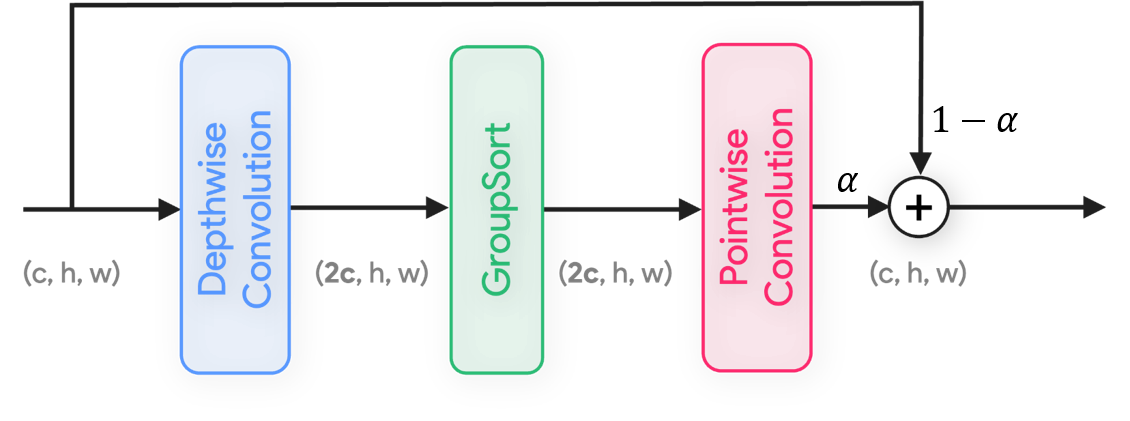
\includegraphics[width=\linewidth]{flash_bcop/figs/illustrations/ortho_block2.png}
            \caption{\textbf{We can construct complex blocks.} These blocks can reduce the number of parameters of our models, thanks to the flexibility of AOC. Lipschitz continuity is guaranteed when $\alpha \in [0, 1]$. }%\thib{todo missing alpha in skip connection}
            \label{fig:imagenet_block}
        \end{subfigure}
        \caption{\textbf{Architecture used for CIFAR-10 accurate setting.} This architecture makes use of its flexibility to allow performance with a limited parameter count. \textbf{Left,} table of the global network architecture. \textbf{Right,} detail of he residual depthwise block.}
        \label{fig:arch_cifar_accurate}
    \end{figure*}

    
    \begin{table}[h]
    \centering
    \small
    \renewcommand{\arraystretch}{1.2}
    \begin{tabular}{lcccc}
        \hline
        \textbf{Hyperparameter} 
        & \makecell{\textbf{CIFAR-10}\\\textbf{Acc.}} 
        & \makecell{\textbf{CIFAR-10}\\\textbf{Rob.}} 
        & \makecell{\textbf{ImageNet}\\\textbf{Acc.}} 
        & \makecell{\textbf{ImageNet}\\\textbf{Rob.}} 
        \\
        \hline
        \textbf{Loss function} 
        & Cosine similarity 
        & \makecell{\cite{prach_almost-orthogonal_2022} \\ $m= 1.5\sqrt{2}$ \\ $\tau=0.125$} 
        & Cosine similarity 
        & \makecell{\cite{prach_almost-orthogonal_2022} \\ $m= 1.5\sqrt{2}$ \\ $\tau=0.125$} 
        \\
        \textbf{Optimizer} 
        & \multicolumn{4}{c}{ScheduleFree \cite{defazio2024roadscheduled}} 
        \\
        \textbf{Learning rate} 
        & $5 \times 10^{-3}$ 
        & $1 \times 10^{-4}$ 
        & $1 \times 10^{-2}$ 
        & $1 \times 10^{-3}$ 
        \\
        \textbf{Batch size} 
        & 1024 
        & 1024 
        & 512 
        & 512
        \\
        \textbf{Epochs}
        & 150 
        & 3000 
        & 90
        & 300
        \\
        \makecell[l]{\textbf{RandAugment}\\\textbf{parameters}} 
        & m=6, n=2
        & m=6, n=1
        & m=7, n=2  
        & None
        \\
        \makecell[l]{\textbf{Random crop}\\\textbf{parameters}} 
        & scale = 0.25
        & scale = 0.5
        & scale = 0.5
        & scale = 0.08
        \\
        \textbf{Hardware} 
        & RTX 3080 $\times$ 1
        & RTX 4090 $\times$ 1
        & RTX 4090 $\times$ 2
        & RTX 4090 $\times$ 2
        \\
        \hline
    \end{tabular}
    \caption{\textbf{Training Hyperparameters for the Four 1-Lipschitz Networks.} 
    ``Acc.'' refers to the high-accuracy setting, and 
    ``Rob.'' refers to the robust setting.}
    \label{tab:hyperparams}
\end{table}


All hyperparameters of the experiments are detailed in \cref{tab:hyperparams}. These parameters were not heavily tuned: the batch size was set to a large value, but we limited it to 1024 to avoid training for too many epochs. This is due to the fact that robust networks seem to benefit more from more training steps rather than larger batch sizes. Once the batch size was set, the learning rate was tuned the following way: by training multiple times for 500 steps, the learning was increased until the accuracy at the end of these 500 steps was maximized, and the final learning rate was set to the largest values before the metrics plateaus.

For robust training, we must control three elements: accuracy, robustness, and generalization. As noted by \cite{prach2024intriguing, bethune_pay_2022}, usual scaling laws do not embrace the fact achieving accuracy and robustness simultaneously comes at the price of generalization. Which can be regained by using larger networks, more data augmentation, and longer train times. To control this phenomenon, we can tune the following 3 elements:
    \begin{itemize}
        \item \textbf{Loss parameters}: Increasing the margin in the loss function helps improve training robustness, but reduces training accuracy.
        \item \textbf{Model size}: Increasing the model size generally improves training accuracy.
        \item \textbf{Data augmentation}: Increasing data augmentation reduces training accuracy but can improve validation accuracy, especially when training accuracy is greater than validation accuracy.
    \end{itemize}

The tuning process then works following these steps:
\begin{enumerate}
    \item start with a given architecture and a low margin $m=0$
    \item increase data augmentation until train accuracy goes below 100\%. The model reached its maximum generalization for this margin.
    \item increase the margin, increase the model size and number of epochs until it reaches 100\% training accuracy.
    \item repeat steps 2. and 3. until the desired robustness is achieved. The target margin is $m=\frac{3}{2}\sqrt{2}$ to match the parameters used by \cite{araujo_unified_2023}. In practical contexts, m should be set to $m = \frac{\epsilon \sqrt{2}}{\alpha L}$ where $\epsilon$ is the targeted robustness radius, L the model's Lipschitz constant and $\alpha$ the scaling factor applied on the data (for instance when standard rescaling is performed) the $\sqrt{2}$ factor comes from the equation in \cref{subsec:certif_rob}.
\end{enumerate}

This explains the drastic difference between standard and robust networks in terms of model sizes and training times. 
\paragraph{Overview of the architectures used}

    \begin{table}%{r}{0.5\textwidth} 
        \centering
        \begin{tabular}{lrl}
            \hline
            \textbf{Layer Type} & \makecell{\textbf{Output}\\\textbf{Shape}} & \textbf{Config} \\
            \hline
            \textbf{Feature Extractor} & & \\ 
            3 x AOC            & [128, 32, 32]  & 3x3 kernel \\
            AOC                & [256, 16, 16]  &  stride=2 \\
            3 x AOC            & [256, 16, 16]  & 3x3 kernel \\
            AOC                & [512, 8, 8]    &  stride=2 \\
            3 x AOC            & [512, 8, 8]    & 3x3 kernel \\
            AOC                & [1024, 4, 4]   &  stride=2 \\
            4 x AOC            & [1024, 4, 4]   & \\
            Flatten            & [8192]         & \\
            \hline
            \textbf{Fully Connected} & & \\
            4 x OrthogonalDense & [1024] & \\
            OrthogonalDense     & [10]   & \\
            \hline
        \end{tabular}
        \caption{\textbf{Architecture of the CIFAR-10 robust network.} unlike other networks, this network has an architecture designed to be similar to the original network from \cite{li_preventing_2019} (with increased width and depth). It follows the original design choices (using circular padding and the absence of global pooling).}
        \label{tab:cifar10_architecture_robust}
     \end{table}

    All the architectures used in this paper aims to illustrate that despite its under-parametrization, AOC allows the construction of expressive architectures. All architectures only use AOC convolutions and standard blocks to ensure that performance can be attributed to the method. As underline in \cite{anil_sorting_2019} it is the combination of orthogonal layer and MaxMin activations that permits the construction of networks with a tight estimation of their Lipschitz constant. We then use MaxMin activation in all of our architectures. The reader interested in building 1-Lipschitz networks that use ReLU activations can refer to the work of \cite{araujo_unified_2023} and \cite{wang_direct_2023}. We describe interactions between AOC and these constructions in \cref{sec:ap_improving_existing}.

    Some of our architectures use skip connections, since those do not construct 1-Lipschitz blocks, we add a learnable factor to correctly ensure the 1-Lipschitzness of the whole network. Given $f_1$ a $l_1$ Lipschitz function and $f_2$ a $l_2$ Lipschitz function, then $f = f_1 + f_2$ is $l_1 + l_2$ Lipschitz. Then the function:
    \[
        y = \frac{\alpha_1 x + f(\alpha_2 x)}{|\alpha_1|+|\alpha_2|}
    \]
    is 1 Lipschitz. This is also true when summing $\alpha_2 f(x)$ instead of $f(\alpha_2 x)$, but the proposed approach allows to control the gradient flowing through $f$. Finally we set $\alpha_1 = 1$ to ensure a better gradient propagation in deep architectures.

\paragraph{CIFAR-10 \cite{krizhevsky2009learning}}
    
    The CIFAR-10 experiments used three distinct networks, the network tailored for accuracy is detailed in \cref{fig:arch_cifar_accurate}, in this setting zero padding is used, with this padding, the layer is 1-Lipschitz and quasi-orthogonal (orthogonal everywhere except for the images border, see \cite{delattre2023efficient, delattre2024spectral} for details). This architecture features a bloc inspired by \cite{trockman_patches_2022} which consists of a depthwise convolution that doubles the number of channels, followed by a MaxMin activation function \cite{anil_sorting_2019} to enhance non-linearity, and a pointwise convolution that reduces the number of channels. These layers are encapsulated within a skip connection featuring a learnable factor to ensure a Lipschitz constant of 1. On the other hand, the robust network has an architecture designed to be as similar as possible to the networks used by \cite{li_preventing_2019} which allows to show the impact of scale on the results. The architecture is detailed in \cref{tab:cifar10_architecture_robust}.
    Finally, the network of the \textit{AOC robust*}, reuses the training recipe of \cite{hu_recipe_2023} with the original convolutions replaced by AOC convolutions (which include downsampling convolutions). The residual connections were removed, and a constant value of $1.15$ replaced the scalar factors. This resulted in a network with a tighter Lipschitz constant evaluation, which resulted in non-optimal training with original loss parameters (the training led to networks that were not accurate enough). Hence, the loss parameters were divided by 10 to make the network more accurate.

    We tested the robust architecture in an accurate setting and vice versa, we observed that the robust architecture was under-performing in the accurate setting, plateauing at 85\% of validation accuracy and 0\% of certified robust accuracy. Similarly, the accurate architecture was underperforming in terms of robustness with only 47\% of certified robust accuracy and 71\% of validation accuracy.
    
    % Each block uses circular padding with a kernel size of 3, ensuring consistency in spatial dimensions throughout the network. This design explores the impact of deep, wide layers combined with orthogonality, aiming to maintain expressiveness while ensuring certifiable robustness.
    % We used the ScheduleFree optimizer \cite{defazio2024roadscheduled} with a learning rate of $1\times10^{-4}$ and no weight decay.


\paragraph{Imagenet-1K \cite{deng2009imagenet}}

    \begin{table}%{r}{0.5\textwidth}
        % \small
        \centering
        \begin{tabular}{lrl}
        \hline
        \textbf{Layer Type}             & \makecell{\textbf{Output}\\\textbf{Shape}} & \textbf{Config} \\ \hline
        Input                           & [224, 224]                 & \\ \hline
        Convolution Layer 1             & [112, 112]               & 5x5 kernel \\ 
        Activation Layer 1              & [112, 112]               & MaxMin \\ \hline
        \textbf{Block 1}                &                               & \\ 
        Residual Depthwise Block x 3    & [56, 56]                 & 5x5 kernel \\ 
        Convolution Layer               & [28, 28]                 & 3x3 kernel \\ \hline
        \textbf{Block 2}                &                               & \\ 
        Residual Depthwise Block x 3    & [28, 28]                 & 5x5 kernel \\ 
        Convolution Layer               & [14, 14]                & 3x3 kernel \\ \hline
        \textbf{Block 3}                &                               & \\ 
        Residual Depthwise Block x 3    & [14, 14]                & 5x5 kernel \\ 
        Convolution Layer               & [7, 7]                  & 3x3 kernel \\ \hline
        \textbf{Block 4}                &                               & \\ 
        Residual Depthwise Block x 3    & [7, 7]                  & 5x5 kernel \\ \hline
        L2 Pooling                      & [1, 1]                  & 3x3 kernel \\ 
        Flatten                         & [2048]                        &  \\ 
        Fully Connected Layer           & [1000]                        &  \\ \hline
        \end{tabular}
        \caption{\textbf{Summary of our architecture used on Imagenet-1K.}}
        \label{tab:splitconcatnet_architecture}
    \end{table}

     The ImageNet-1K experiment follows the hyperparameter configuration detailed in Table~\ref{tab:hyperparams}. The two architectures utilized in this study exhibit a high degree of similarity, with their structural differences illustrated in Figure~\cref{tab:splitconcatnet_architecture}. Both architectures incorporate the fundamental block described in Section~\cref{fig:imagenet_block}.

    The primary distinction between the accurate and robust settings lies in the architectural modifications aimed at enhancing robustness. Specifically, the robust architecture employs L2-normalized pooling~\cite{boureau2010theoretical} and circular padding, both of which contribute to improved resilience against adversarial perturbations. Furthermore, inspired by~\cite{trockman_patches_2022}, the convolutional blocks in the robust model utilize larger kernel sizes to capture a broader spatial context.
     % We leveraged the flexibility of our layer to design more complex blocks tailored for ImageNet1K. Each block consists of a depthwise convolution that doubles the number of channels, followed by a MaxMin activation function \cite{anil_sorting_2019} to enhance non-linearity, and a pointwise convolution that reduces the number of channels. These layers are encapsulated within a skip connection featuring a learnable factor to ensure a Lipschitz constant of 1, represented by $y = \alpha x + (1-\alpha) f(x)$ (where $\alpha \in [0, 1]$). A visual description can be found in \cref{fig:imagenet_block}. The entire architecture consists of a sequence of such blocks interleaved with strided convolutions, an exhaustive description of the architecture is provided in \cref{tab:splitconcatnet_architecture}.

    % \begin{figure}%[h]
    %     \centering
    %     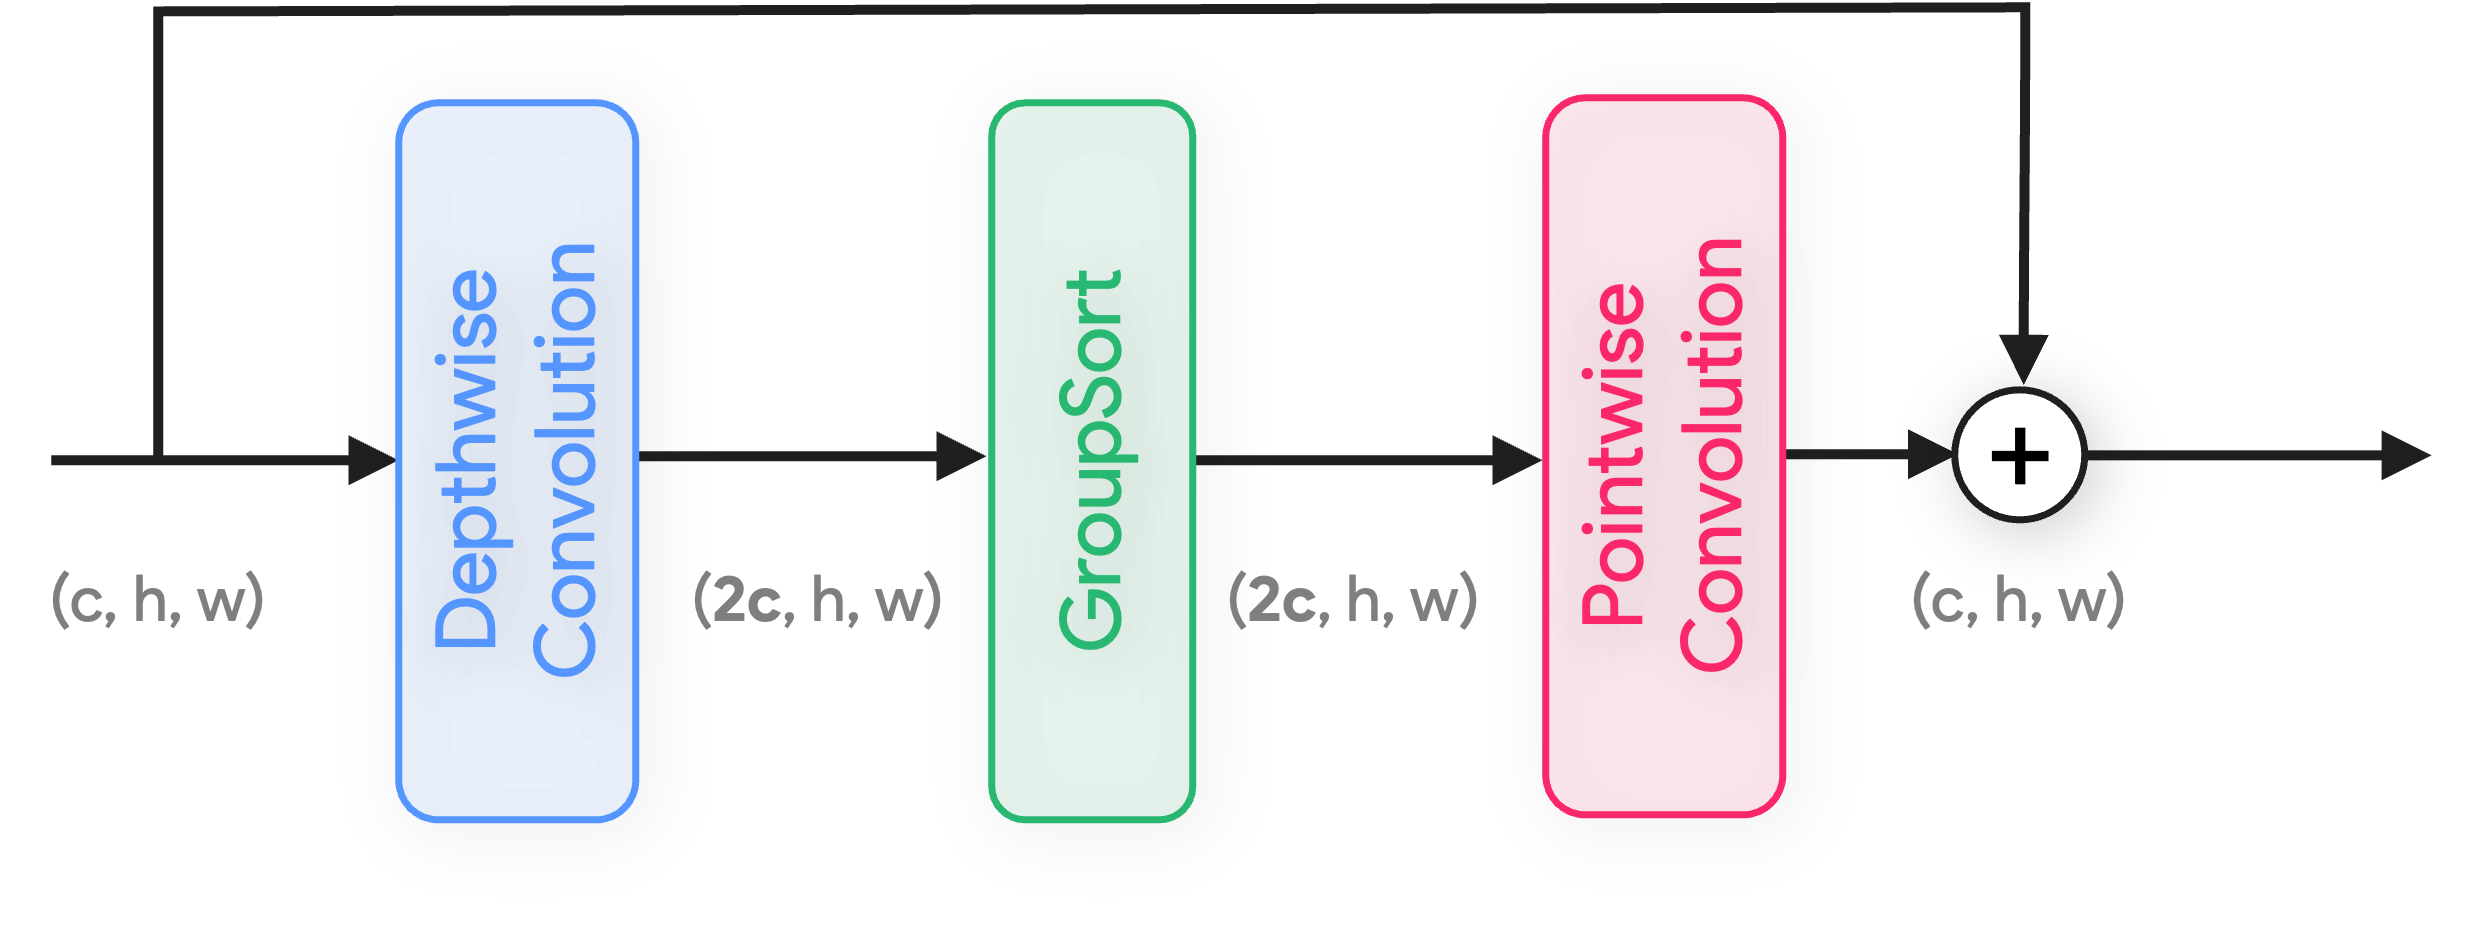
\includegraphics[width=0.45\linewidth]{flash_bcop/figs/illustrations/ortho_block.png}
    %     \caption{\textbf{We can construct complex blocks.} These blocks can reduce the number of parameters of our models, thanks to the flexibility of AOC.}\thib{todo missing alpha in skip connection}
    %     \label{fig:imagenet_block}
    % \end{figure}

% \thib{

% \paragraph{Expressive power.}

%     \todo{The reviewer would like to encourage adding explanations for the undeclared letters such as the binary loss threshold eps=36/255  (to explain the so-called “provable accuracy”), the hinge loss margin m=72/255,1.5/2 and how these numbers are tuned to avoid confusion}
    
%     The most straightforward way to evaluate the expressiveness of our layers is to apply them to classification problems. It is well known that 1-Lipschitz constrained networks face an inherent trade-off between accuracy and robustness \cite{bethune_pay_2022}. Fortunately, this trade-off can be controlled using the loss's parameters: we can then evaluate our model at two different points of the trade-off to show that it can achieve both a decent accuracy and a decent certifiable robustness. Our approach is not expected to improve the expressiveness of the original building blocks like BCOP and RKO. However, authors of \cite{prach_1-lipschitz_2023} observed that improvement of the state of the art in certifiable adversarial robustness comes along with larger architectures and longer training times. Therefore, given the same computational budget, we can expect that our efficient implementation unlocks larger networks and more training steps, which in turn should improve final performance.
    
%     In our evaluation on CIFAR10, we scaled the network from \cite{li_preventing_2019} to be wider and deeper: our model consists of 4 blocks of 3 convolutions interleaved with strided convolutions where the number of channels was increased by a factor of 2x. The head of the network consists of 5 dense layers. The number of channels of the first block was set to 128, and the size of dense layers was set to 1024. A detailed description of our training setting can be found in  \cref{sec:ap_training_details}. We changed the loss to the CrossEntropy loss as in \cite{prach_almost-orthogonal_2022}, which allows us to control the accuracy/robustness trade-off. We did not use techniques such as last layer normalization, certificate regularization \cite{singla_skew_2021}, or DDPM augmentation \cite{hu_recipe_2023} to obtain our results, which are shown in the first part of \cref{tab:robust_cifar10}.
%     We controlled three elements during the hyper-parameter tuning process:
%     \begin{itemize}
%         \item \textbf{Loss parameters}: Increasing the margin in the loss function helps improve training robustness, but reduces training accuracy.
%         \item \textbf{Model size}: Increasing the model size generally improves training accuracy.
%         \item \textbf{Data augmentation}: Increasing data augmentation reduces training accuracy but can improve validation accuracy, especially when training accuracy is greater than validation accuracy.
%     \end{itemize}
    
%     The tuning process begins with a given model. We first tune the learning rate and increase the margin in the loss function to improve robustness until training accuracy drops below 100\%. Then, we increase the model size and apply more data augmentation until training accuracy falls below validation accuracy.
    
    
%     % The most straightforward way to evaluate the expressiveness of our layer is to apply it to classification problems. It is well known that 1-Lipschitz constrained networks face an inherent trade-off between accuracy and robustness \cite{bethune_pay_2022}. Fortunately this trade off can be controlled using the loss parameters: we can then evaluate that our model at two different points of the trade-off, to show that it can achieve both a decent accuracy and a decent certifiable robustness. Our approach is not expected to improve the expressiveness of the original building blocs like BCOP and RKO. However, authors of \cite{prach_1-lipschitz_2023} observed that improvement of the state of the art in certifiable adversarial robustness comes along larger architectures and longer training times. Then we can expect that, given the same computational budget, our efficient implementation unlock larger networks and more training steps which in turn, improve final performances. %For reference, the total cost of all experiments ran on CIFAR10, including, architecture search and hyper-parameters tuning amount to 15 GPU days on a consumer RTX4090.
%     % %we first confirmed that our approach did not introduce any regression by replicating the experiment from \cite{li_preventing_2019}.
%     % \paragraph{Evaluation on CIFAR10:} We scaled the network from \cite{li_preventing_2019} to be wider and deeper: our model which consist in 4 block of 3 convolutions interleaved with strided convolutions where the number of channels were increased by a factor of 2x. The head of the network consists in 5 dense layers. The number of channels of the first block were set to 128 and the size of dense layers were set to 1024. We changed the loss to the CrossEntropy loss as in \cite{prach_almost-orthogonal_2022}, which allows the control of the accuracy/robustness tradeoff. Although the network were significantly larger, we could increase the batch to 1024 on a single GPU. Results are shown in the first part of  \cref{tab:robust_cifar10}.

%     In our evaluation on ImageNet1K, we leveraged the flexibility of our layers to design more complex blocks. A comprehensive description of the whole architecture is given in \cref{sec:ap_training_details}. Each block consists of a depthwise convolution that doubles the number of channels, followed by a MaxMin activation function \cite{anil_sorting_2019}, and a pointwise convolution that reduces the number of channels. These layers are encapsulated within a skip connection featuring a learnable factor to ensure a Lipschitz constant of 1. The network was constructed by repeating these blocks, using strided convolutions to progressively reduce the spatial dimensions while increasing the channel dimensions. The architecture ends with L2 Norm Pooling \cite{boureau2010theoretical}, followed by a single dense layer for classification.
%     We evaluated the network under two distinct settings. In the first setting, we used Cosine similarity to maximize accuracy, focusing on achieving optimal performance for clean data. In the second setting, we applied categorical cross-entropy with a margin of $m=1.5\sqrt{2}$ to emphasize robustness against adversarial examples. The results for both settings are presented in the second part of \cref{tab:robust_cifar10}.


%     % \paragraph{Evaluation on Imagenet 1K:} We leverage the flexibility of our layer to design more complex blocs. The block we designed consist in a depthwise convolution that double the number of channels followed by a MaxMin \cite{anil_sorting_2019} activation and a pointwise convolution that reduce the number of channels. These layers are encapsulated in a skip connection with a learnable factor that ensure a Lipschitz constant of 1: $y = \alpha x + (1-\alpha) f(x)$ (with $\alpha \in [0, 1])$. We repeated these blocks and added strided convolutions to reduce spatial dimension and increase channels dimension. The network uses an L2 Norm Pooling followed by a single dense layer for classification. In the first setting, we used the Cosine similarity to maximize accuracy, and in the second setting we used the categorical cross-entropy with a margin $m=1.5\sqrt{2}$ to measure robustness. Results are shown in the second part of  \cref{tab:robust_cifar10}.
    

% }

\subsection{Scalability experiment}\label{ap:scale_xp}

    Experiments were conducted on a minimally modified ResNet-34 architecture, chosen for its compatibility with various orthogonal layers and its status as a standard benchmark for ImageNet training. The transition blocks were replaced by a single, strided convolution to maintain simplicity and ensure compatibility with existing orthogonal layers. For each method, we measured the average training and testing times over 100 batches and recorded peak memory consumption. Starting with a batch size of 128, we doubled the batch size incrementally until encountering an out-of-memory error. Each method’s performance was compared to a standard convolution baseline, with results reported as overhead percentages.

    To ensure a fair comparison, the hyperparameters of SOC and Cayley were set to their default values. We adjusted the number of Björck iterations to the same values for BCOP and AOC. While originally set to 20 iterations, our unit testing scheme (see  \cref{ap:unit_testing}) shows that 12 iterations are sufficient to ensure a stable rank \cite{sanyalstable} of 99.9\% of the full rank. Finally, standard \texttt{Conv2D} is used with circular padding to evaluate the overhead induced by our parametrization rather than the overhead induced by the padding.

    We did not include non-orthogonal methods such as AOL, SLL, CPL and RKO \cite{prach_1-lipschitz_2023, araujo_unified_2023, meunier_dynamical_2022, serrurier_achieving_2021} as those are expected to be faster than AOC that add a stronger constraint. The continuum between orthogonal and non-orthogonal methods could be explored by reducing the number of Björck and Bowie iterations. However, the correct way to explore this should be with an experiment that grasp the 3 main aspects of those methods: speed (time per batch), trainability (number of batches to reach certain accuracy) and performance (final accuracy/robustness). This is beyond the scope of this work, and the work of \cite{prach_1-lipschitz_2023} is a relevant track to explore this question. %\thib{Todo: run an experiment with non-orthogonal methods and show that we compete with those}


\section{Reproducing the results from BCOP paper}\label{ap:repoducing_bcop}
    
    As mentioned earlier, AOC is built on top of components like BCOP and RKO. Hence, any accuracy gain must come from the fact that our implementation allows larger networks and more training steps within the same compute budget. To illustrate this, we reproduced the baseline results from \cite{li_preventing_2019} and switched the implementation to ours. Results are shown in \cref{tab:bcop_replication}. We can observe a notable difference in performance between the original implementation and ours. This is due to the difference in the parametrization of strided convolutions: the original paper uses invertible downsampling to emulate striding followed by a standard convolution whose number of input channels is multiplied by $s^2$, such convolution has a $s^2\times$ more parameters than the proposed AOC strided convolution.
        \begin{table}%{r}{0.6\textwidth} 
        \centering
            \begin{tabular}{rrr}
            \toprule
                    Models & \makecell{Acc-\\uracy} &  \makecell{Provable \\ Accuracy \\ $\epsilon = \frac{36}{255}$}  \\
            \midrule
              BCOP - Small net (original seeting) & 72.2 & 58.26 \\
              AOC - Small net (all optimizations) & 62.3 & 49.18 \\
              AOC - Small net (opt in \cref{fig:method_simplify} removed) & 71.8 & 58.25 \\
              \hline
              AOC - Large net (all optimizations) & 74.0 & 64.33 \\
            \bottomrule
            \end{tabular}
        \caption{\textbf{Mitigating AOC limitations in small scale setting}: as AOC uses less parameters for strided convolutions, this can impact its expressive power in small scale setting. However, by removing the optimization in \cref{fig:method_simplify} this increase the number of parameters enough to correct this issue. Results from \cref{tab:robust_cifar10} added for reference.}
        \label{tab:bcop_replication}
    \end{table}
     This is accentuated by the specific small architecture used in BCOP paper (and reproduced in this experiment) which has 84\% of the convolutional layers parameters that are located in strided convolutions.Also, invertible down-sampling has a $2 \times 2$ receptive field, which increases the global convolution's receptive field. However, when we remove the optimization depicted in \cref{fig:method_simplify} and only resort to the parametrization described in \cref{fig:method_bigpic}, the increase in the number of parameters results in improved results close to the results of the original paper. This observation is non-trivial since this modification is not equivalent to the original implementation: instead of parametrizing a $c_o \times 4 \, c_i \times k \times k$ AOC parameterized one $\max(c_i, \frac{c_o}{s^2}) \times c_i \times k-s+1 \times k-s+1$  and one $c_o \times \max(c_i, \frac{c_o}{s^2}) \times s \times s$ kernels which are much smaller.

    We recall that all the results of this paper were obtained with the optimization in \cref{fig:method_simplify}. We evaluated the unoptimized version in the same context as in \cref{tab:comparison_overhead} and found, for a batch size of 512, a slowdown of $1.21 \times $ in train time (instead of $1.13\times$) and no notable increase in train memory consumption.

    Finally, it is worth noting that the optimization depicted in \cref{fig:method_simplify} should not affect the expressive power if we were able to parameterize the complete set of orthogonal convolutions.